%% 
%% Copyright 2019-2024 Elsevier Ltd
%% 
%% This file is part of the 'CAS Bundle'.
%% --------------------------------------
%% 
%% It may be distributed under the conditions of the LaTeX Project Public
%% License, either version 1.3c of this license or (at your option) any
%% later version.  The latest version of this license is in
%%    http://www.latex-project.org/lppl.txt
%% and version 1.3c or later is part of all distributions of LaTeX
%% version 1999/12/01 or later.
%% 
%% The list of all files belonging to the 'CAS Bundle' is
%% given in the file `manifest.txt'.
%% 
%% Template article for cas-sc documentclass for 
%% double column output.

\documentclass[a4paper,fleqn]{cas-sc}

% If the frontmatter runs over more than one page
% use the longmktitle option.

%\documentclass[a4paper,fleqn,longmktitle]{cas-sc}

% =====================================
%% Custom commands
%\usepackage[numbers]{natbib}
%\usepackage[authoryear]{natbib}
\usepackage[authoryear,longnamesfirst]{natbib}
\newcommand{\defeq}{\stackrel{\scalebox{0.5}{\ensuremath{\mathsf{\,def}}}}{=}}
\usepackage{moreverb,xurl}
\usepackage{booktabs,makecell,threeparttable,tabularx,array}
\usepackage{multirow} % for \multirow in tables
\usepackage{siunitx}  % for S column type (numeric alignment)

%% Graphics / utilities
\usepackage{graphicx}  % \scalebox
\usepackage{etoolbox}  % \csdef
\usepackage{xspace}    % \xspace
\usepackage{placeins}  % keep result floats close to their discussion

%% Theorems
\usepackage{amsthm}
\newtheorem{observation}{Observation}
\newtheorem{assumption}{Assumption}
\newtheorem{proposition}{Proposition}
\newtheorem{deploymentrule}[proposition]{Rule}
%% Algorithms
\usepackage{algorithm}
\usepackage{algorithmic} % provides \REQUIRE/\ENSURE/\STATE etc.

%% Subfigures
\usepackage{subcaption}

%% PGF plots
\usepackage{pgfplots}
\pgfplotsset{compat=1.18}

%% Special math fonts
\DeclareMathAlphabet{\pazocal}{OMS}{zplm}{m}{n}

%% Hyperlinks (should be loaded last)
\usepackage{hyperref}

% for revising
\usepackage{ulem} % 提供 \sout 命令
\newcommand{\keepcomment}{0} % 1 - Keep comments, 0 - Hide comments
\ifnum\keepcomment=1
	\usepackage[colorinlistoftodos,textsize=scriptsize]{todonotes} % todo
    \newcommand{\stkout}[1]{\ifmmode\text{\sout{\ensuremath{#1}}}\else\sout{#1}\fi}
    % \long + {\color{red}#3} group lets the new-text argument span multiple
    % paragraphs / contain \paragraph and \subsection (block-level revisions).
    \long\def\rev#1#2#3{\textcolor{blue}{\begin{scriptsize}{#1}\end{scriptsize}\stkout{#2}}{\color{red}#3}}
\else
	\long\def\rev#1#2#3{\ignorespaces#3\ignorespaces\unskip}
	\usepackage[disable]{todonotes} % todo
\fi

\newcommand\todoi[1]{\todo[inline]{#1}}

\newcolumntype{Y}{>{\centering\arraybackslash}X}

% for figure
\usepackage{pgfplots}
\usepackage{subcaption}
\pgfplotsset{compat=1.18}
% =====================================

%%%Author macros
\def\tsc#1{\csdef{#1}{\textsc{\lowercase{#1}}\xspace}}
\tsc{WGM}
\tsc{QE}
%%%

% Uncomment and use as if needed
%\newtheorem{theorem}{Theorem}
%\newtheorem{lemma}[theorem]{Lemma}
%\newdefinition{rmk}{Remark}
%\newproof{pf}{Proof}
%\newproof{pot}{Proof of Theorem \ref{thm}}

\begin{document}
\shorttitle{Supplementary material: Public transport line redesign}
\shortauthors{Guo et al.}
\title [mode = title]{Supplementary material: Predict-then-Optimize Framework for Public Transport Line Redesign under Fluctuating Traffic Conditions}
\begin{abstract}
This document provides supplementary derivations, algorithmic and evaluation details, and additional results for the conference paper.
\end{abstract}
\maketitle
\appendix

\section{Additional details of the solution algorithm}
\subsection{Solution Encoding}\label{sec:encoding}

% ********************* 线路组成
In the proposed NSGA-III method, each PT line $\ell$ is represented as an ordered simple path
$p_\ell = (i_1, i_2, \dots, i_{n_\ell})$ with $i_j \in \pazocal{N}$ and no repeated nodes, which enforces acyclicity by construction as required by the line-structure and fleet constraints.
PT lines may either be constructed from \textit{scratch} or obtained by \textit{reconstructing bus routes from the existing network}.
Starting from a current node $i$, the algorithm maintains a visited-node set $\pazocal{V}_{\text{visited}}^\ell$ and defines the set of feasible candidates as
$
\pazocal{N}_{\text{unvisited}}(i)
=
\{\, j \in \pazocal{N}(i) : j \notin \pazocal{V}_{\text{visited}}^\ell \,\},
$
which is used whenever a new path segment needs to be generated.
For lines constructed from scratch, the path is iteratively extended by selecting the next node $j \in \pazocal{N}_{\text{unvisited}}(i)$ according to the travel-time weighted probability
\begin{equation}
\label{eq:node-addition-probability}
\mathbb{P}(j \mid i)
=
\frac{1/t_{ij}}{\sum_{k\in\pazocal{N}_{\text{unvisited}}(i)} 1/t_{ik}},
\end{equation}
which favors temporally efficient connections while preserving stochastic exploration.
%
When a line is derived from the existing network, local modifications are applied by replacing a selected route segment with an alternative feasible path that preserves the original endpoints.

% ********************* 车辆分配
Simultaneously, vehicle allocation is managed by assigning integer variables $n^\ell$ to each line. 
%
During initialization,
each line is pre-allocated one vehicle to guarantee basic service availability.
The remaining $V_{\max}-|\pazocal{L}|$ vehicles are then distributed across
lines proportionally to their initial one-way travel times $t^\ell$ (computed based on nominal link travel times $t_{ij}$).
% and encoded as part of the initial chromosome representation,
% with integer rounding ensuring
% $\sum_{\ell\in\pazocal{L}} n^\ell = V_{\max}$.
% %
% Subsequently, fleet allocation is jointly evolved with line topologies through
% crossover and mutation operators, and waiting times $w^\ell$
% (defined in Eq.~\eqref{eq:headwayTime}) are updated whenever $n^\ell$ is modified.

% ------------------------------------------------------
% ============================ 4.2
% ------------------------------------------------------
\subsection{Evolutionary Search Procedure}
\label{sec:search}

Each individual encodes a complete PT network design, comprising a set of line path representations and the associated vehicle allocations.
Starting from an initial population, the algorithm evolves solutions in a generational manner.
At each generation, offspring are produced through selection, variation, and evaluation, followed by the NSGA-III reference-point-based \textit{environmental selection}, which prioritizes non-dominated solutions while maintaining diversity along the Pareto front.
The conference paper summarizes the overall procedure.

% -------------------- 4.2.1
\subsubsection{Population Initialization}
\label{sec:init_population}

During population initialization ,
each individual is generated using the line construction rules described in $\S$~\ref{sec:encoding}.
PT lines are either constructed from scratch or obtained by locally perturbing routes reconstructed from the existing network.
Given a set of lines, vehicle allocations are initialized by assigning one vehicle to each active line to guarantee basic service availability.
The remaining fleet is then distributed across lines according to the chromosome encoding scheme described in $\S$~\ref{sec:encoding}, ensuring $\sum_{\ell \in \pazocal{L}} n^\ell = V_{\max}$.

To expedite initialization, candidate solutions are screened via a \textbf{connectivity check} on the undirected graph induced by
$\pazocal E_{\text{PT}} = \bigcup_{\ell\in\pazocal L} \pazocal E_\ell$,
i.e., the union of all active line edges in $\pazocal G_{\text{PT}}$.
By employing a Union--Find data structure, we efficiently identify connected components, and verify that, for every OD pair $k\in\pazocal K$, the origin $o_k$ and destination $d_k$
belong to the same connected component (which implies that it is possible to go from one to the other).
% This screening step avoids the computational overhead of full shortest-path evaluations during population initialization.
%
The procedure is repeated until $\textit{PopSize}$ individuals (i.e., PT network structures) are generated that satisfy:
(i)~structural validity (lines are simple-paths, with no branches nor cycles),
(ii)~connectivity-based serviceability, i.e., all OD pairs $k\in\pazocal K$ are connected within $\pazocal G_{\text{PT}}$,
and (iii)~similarity, i.e., individual~$\pazocal G_\text{PT}$ is not extremely different from original PT network~$\pazocal G_\text{PT}^\text{org}$, i.e., the Jaccard similarity index must be above threshold $J_{\min}$.
These criteria enforce a necessary (but not sufficient) condition for OD reachability; full feasibility and network performance are subsequently evaluated using the decode-and-assign objective.

% -------------------- 4.2.2
\subsubsection{Crossover Operation}\label{sec:crossover}

With probability $P_c$, a crossover operator is applied to two parent solutions, denoted as parents $A$ and $B$.
Each solution consists of a fixed set of PT lines, where each line is treated as a basic inheritance unit characterized jointly by its bus route topology and vehicle allocation.
The crossover exchanges complete lines between parents as the primary recombination mechanism; any subsequent modifications are limited to feasibility restoration.

Line inheritance is governed by a binary selection mask $\boldsymbol{\xi}=(\xi_\ell)_{\ell\in\pazocal{L}}$, where each component is independently drawn as $\xi_\ell \sim \mathrm{Bernoulli}(0.5)$,
so that both parents are treated symmetrically and structural diversity is promoted at the line level.
%
Given $\boldsymbol{\xi}$, the offspring design is defined by block-wise inheritance:
\begin{align}
(e_{ij}^\ell)^{\text{off}}
&=
\xi_\ell (e_{ij}^\ell)^{A} + (1-\xi_\ell)(e_{ij}^\ell)^{B},
&& \forall \ell\in\pazocal{L},\ (i,j)\in\pazocal{E},
\label{eq:crossover_edges}\\
(n^\ell)^{\text{off}}
&=
\xi_\ell (n^\ell)^{A} + (1-\xi_\ell)(n^\ell)^{B},
&& \forall \ell\in\pazocal{L}.
\label{eq:crossover_fleet}
\end{align}
Whenever a line topology is inherited from a parent, its vehicle allocation is inherited jointly, thereby preserving the coupling between bus route geometry and service frequency.
% No interpolation across different line structures is performed.

% If any inherited line becomes structurally infeasible (e.g., disconnected or discontinuous), a localized repair mechanism is triggered using a feasibility-oriented repair procedure.
If any inherited line becomes structurally infeasible (e.g., disconnected or discontinuous), a feasibility-oriented restoration operator is applied to recover a valid simple-path representation using a feasibility-oriented repair procedure.
% Repairs are applied only to the affected lines and only when infeasibility is detected, by reconnecting disrupted segments using deterministic or randomized Breadth-First Search (BFS) on the substrate graph.
% This repair step is strictly feasibility-oriented and does not optimize route cost or passenger travel time.
%
Finally, fleet constraints ($n^\ell \ge 1$ for all active lines and $\sum_{\ell\in\pazocal{L}} n^\ell = V_{\max}$) are enforced via minimal $\pm 1$ adjustments on a small subset of lines.
This correction is a feasibility projection and is not guided by objective improvement.
% -------------------- 4.2.3
\subsubsection{Mutation Operation}\label{sec:mutation}

With probability $P_m$, a mutation perturbs a single line $\ell$ via local structural modifications, including node insertion, node deletion, or segment reconnection.
These operations introduce stochastic variations in line topology while preserving the overall chromosome structure.
%
If the mutation results in a disconnected or discontinuous line,
feasibility is restored by reconnecting the affected segments using a feasibility-oriented repair procedure.
This repair step is feasibility-oriented and does not explicitly consider objective values.
%
Finally, global fleet conservation ($\sum_{\ell\in\pazocal{L}} n^\ell = V_{\max}$)
is enforced in the same manner as described in \S~\ref{sec:crossover}.

% -------------------- 4.2.4
\subsubsection{Environmental Selection}\label{sec:env_selection}
After offspring generation, parent and offspring populations are merged and ranked via non-dominated sorting.
%
Environmental selection follows the standard NSGA-III mechanism, employing a set of reference points $N_\text{ref}$ to maintain population diversity~\citep{deb2014nsga3}.\footnote{The implementation details are provided in App.~\ref{A.Evolution}.}
% ------------------------------------------------------
% ============================ 4.3
% ------------------------------------------------------


% --------------------------------------------------- 
% --------------------------------------------------- Appendix 1_Proof of Proposition
% ---------------------------------------------------

\section{Proof and discussion of pairwise stability}
\label{app:temporal_stability_proof}

For any two redesigns, $J(E^{(k)},E^{(k+n)})\geq J(E^{(k)},E^{(0)})+J(E^{(k+n)},E^{(0)})-1$. This is a conditional bound and does not impose a minimum overlap by itself.

\paragraph{Proof.}
Setting $A=\pazocal{E}^{(k)}$, $B=\pazocal{E}^{(0)}$, and $C=\pazocal{E}^{(k+n)}$.
The Jaccard distance between two sets $X$ and $Y$ is
\[
d_J(X,Y)=1-\frac{|X\cap Y|}{|X\cup Y|}=1-J(X,Y).
\]
Levandowsky and Winter~\citep{levandowsky1971distance} noted that this
dissimilarity measure satisfies the triangle inequality on finite sets,
so that $d_J$ may be regarded as a distance function. Hence,
\[
d_J(A,C)\le d_J(A,B)+d_J(B,C).
\]
Substituting $d_J(X,Y)=1-J(X,Y)$ into the above inequality yields
\[
1-J(A,C)
\le [\,1-J(A,B)\,]+[\,1-J(B,C)\,],
\]
which is equivalent to
\[
J(A,C)\ge J(A,B)+J(B,C)-1.
\]
\rev{zg}{, gives the desired result.}{which gives the desired result.}\hfill$\blacksquare$

\paragraph{Remark.}
\rev{zg}{This implies that if two consecutive designs exhibit a similarity of $\geq 90\%$ relative to the original (consistent with our numerical results), the similarity between these two consecutive designs is guaranteed to be at least 80\%.}{For example, if two designs each have similarity of at least 90\% to the original, their mutual similarity is at least 80\%. This conditional example does not assert that every reported design meets the 90\% threshold.}
%
% \rev{zg}{}{
% The crucial point is that, because the structural objective $Z_3$ is measured against the \emph{original} network $\pazocal{E}^{(0)}$ at \emph{every} step rather than against the preceding design, the right-hand side does not depend on the gap $n$. Variability therefore does not accumulate or propagate as the day progresses: the similarity between redesigns one hour apart and the similarity between redesigns twelve hours apart obey the \emph{same} lower bound. While the worst-case guarantee $2J_{\min}-1$ is loose (and vacuous at $J_{\min}=0.5$), the empirically observed similarity to the original network is much higher than $J_{\min}$: Tables~\ref{tab:routeNumberCV} and~\ref{tab:stop_skipping_comparison} report route overlaps of roughly $0.77$--$0.90$, which by the inequality above guarantees $J(\pazocal{E}^{(k)},\pazocal{E}^{(k+n)}) \ge 0.54$--$0.80$ between \emph{any} two redesigns of the day. The hourly monitoring policy (\S\ref{sec:timeframe}), which resets the network to $\pazocal{G}_\text{PT}^\text{org}$ whenever deviations fall within tolerance, provides a further safeguard against long-term drift.}
% --------------------------------------------------- 
% --------------------------------------------------- Appendix 2_log_normal
% --------------------------------------------------- 
\section{Stochastic Modelling of Travel Times and Prediction Errors}

% ================================ A.1
\subsection{Parameter Derivation for Log-Normal Distribution}\label{Appendix:log_normal}

\paragraph{Log-normal parameter derivation.}
For a lognormal random variable $X \sim \mathrm{LogNormal}(\mu,\sigma^{2})$,  
the median is $\mathrm{Med}(X)=\exp(\mu)$, so specifying the median $m$ yields
\[
\mu = \ln(m).
\]

The mean and variance of $X$ are
\[
\mathrm{E}[X] = \exp\!\left(\mu + \tfrac{1}{2}\sigma^{2}\right),
\qquad
\mathrm{Var}(X) = \bigl(\exp(\sigma^{2}) - 1\bigr)\exp\!\left(2\mu + \sigma^{2}\right).
\]
Hence the coefficient of variation is
\[
\begin{aligned}
cv
&= \frac{\sqrt{\mathrm{Var}(X)}}{\mathrm{E}[X]} \\
&= \frac{\sqrt{\bigl(\exp(\sigma^{2}) - 1\bigr)\exp(2\mu + \sigma^{2})}}
        {\exp(\mu + \tfrac{1}{2}\sigma^{2})} \\
&= \sqrt{\exp(\sigma^{2}) - 1}.
\end{aligned}
\]

Equating this expression with the prescribed value of $cv$ gives
\[
cv^{2} = \exp(\sigma^{2}) - 1
\qquad\Longrightarrow\qquad
\sigma^{2} = \ln\!\bigl(1 + cv^{2}\bigr)
\qquad\Longrightarrow\qquad
\sigma = \sqrt{\ln\!\bigl(1 + cv^{2}\bigr)}.
\]
\hfill$\blacksquare$

% ================================ A.2
\subsection{\rev{zg}{}{Traffic Speed Prediction and Error Estimation}}\label{A2}

To generate realistic stochastic prediction errors, we employ the Diffusion Convolutional Recurrent Neural Network (DCRNN) \citep{li2017diffusion} to model spatiotemporal traffic dependencies. Two benchmark datasets are utilized: \textbf{METR-LA} (4 months of highway data from 207 sensors) as a proxy for Mandl’s network, and \textbf{Q-Traffic} (61 days of Beijing 6th Ring Road segments) for the real-world case study. We split both datasets, chronologically,  as recommended by \cite{li2017diffusion} and \cite{lu2022graph}, respectively: We train each prediction model on the first part of the chronologically ordered
data and measure prediction errors on the last part, i.e., the test set.
Table~\ref{tab:prediction_error} reports the one-hour-ahead prediction errors
used in our experiments.

% ----------------- table_predERROR
\begin{table}[htbp!]
\centering
\caption{One-hour-ahead prediction error on benchmark datasets.}
\label{tab:prediction_error}
\begin{tabular}{llcc}
\hline
Dataset & Model & MAE & RMSE \\
\hline
\multirow{2}{*}{METR-LA}
& DCRNN & 3.590 & 7.607 \\
& MTGNN & 3.490 & 7.230 \\
\hline
\multirow{2}{*}{Q-Traffic}
& DCRNN & 3.932 & 6.030 \\
& MTGNN & 2.973 & 4.742 \\
\hline
\end{tabular}
\end{table}
% ----------------- table_predERRORend

The prediction models output traffic speeds. Since the downstream public-transport redesign model operates on travel times, the extracted prediction residuals must be expressed in travel-time space. If a link length $d$ is available, the realized and predicted travel times are $T=d/v$ and $\hat T=d/\hat v$, respectively. 
%
The corresponding log-relative travel-time residual is therefore $\eta=\log(\hat T)-\log(T)$. For a fixed link length, this is equivalently written as $\eta=\log(v)-\log(\hat v)$, since the length term cancels out algebraically.
% ~\footnote{A short derivation is provided in App.~\ref{app:speed_to_time_log_residual}.} 
%
This equivalence is particularly useful for \textbf{METR-LA}, where reliable segment lengths are not directly available for all sensor pairs. In this case, we compute the travel-time log-relative residual directly from the observed and predicted speeds. For \textbf{Q-Traffic}, where segment lengths are explicitly provided, the same residual can be obtained either after converting speeds into travel times or directly through the equivalent speed-based expression. The resulting residual pool is then used to generate noisy travel-time forecasts as described in App.~\ref{A3}.



% -----------------------------
% -----------------------------
% -----------------------------
% ================================ A.3
\subsection{\rev{zg}{}{Empirical Log-Relative Residual Sampling for Travel-Time Prediction}}\label{A3}

We pool all empirical prediction residuals on the test sets, across links and time steps, to construct a representative empirical error pool. Since the downstream experiments transfer prediction errors across links and networks with different travel-time scales, we sample log-relative residuals rather than absolute residuals. Specifically, for each realized travel time $T$ and its prediction $\hat T$, we define $\eta=\log(\hat T)-\log(T)=\log\left(\hat T/T\right)$.
%
This log-ratio formulation is appropriate for heteroscedastic prediction errors whose magnitude scales with the level of the predicted variable~\citep{Tofallis2015}; in our setting, this is consistent with traffic scenarios in which the coefficient of variation changes the scale of realized travel times. 
% 适合误差随变量尺度增长的 heteroscedastic 情况
%
Finally, independent samples $\eta_{ij}^{\omega}$ are drawn with replacement from this empirical pool for each link $(i,j)$ and scenario $\omega$. Given the realized travel time $t_{ij}^{\omega}$ generated under the prescribed traffic-variability level, the corresponding additive travel-time error is defined as $\epsilon_{ij}^{\omega}=t_{ij}^{\omega}\left(\exp\!\left(\alpha\eta_{ij}^{\omega}\right)-1\right)$. The predicted link travel times~$\hat t_{ij}^{\omega}$, used to make network-design decisions, are then computed by adding $\epsilon_{ij}^{\omega}$ to the actual travel time~$t_{ij}^{\omega}$, as $\hat t_{ij}^{\omega}=t_{ij}^{\omega}+\epsilon_{ij}^{\omega}$. We do this in both Mandl and Beijing scenarios.

Moreover, because errors are sampled independently for each link and scenario, this first-order model abstracts away the spatial and temporal correlation of real forecast errors, such as corridor-level or incident-level common shocks. The reported results should therefore be read as an evaluation under sampled independent empirical residual scenarios, and correlation-aware forecast-error modeling remains an important extension. \rev{zg}{}{Because the simulated forecasts are constructed from realized times, this controlled error experiment does not itself validate a live, ex-ante forecasting system.}

\begin{equation}
\hat t_{ij}^{\omega} = t_{ij}^{\omega}
+
\epsilon_{ij}^{\omega}, \
%
\epsilon_{ij}^{\omega} =
t_{ij}^{\omega}
\left(
\exp\!\left(\alpha\eta_{ij}^{\omega}\right)-1
\right)
\label{eq:predTRAVEL_appendix}
\end{equation}


% ----------------------

\paragraph{Diagnostic check on traffic variability.}
For the Mandl experiments, we further report the realized-to-nominal travel-time ratio
$R_{ij}^{\omega}=t_{ij}^{\omega}/t_{ij}^{0}$, where $t_{ij}^{0}$ is the nominal link travel time and $t_{ij}^{\omega}$ is the realized travel time under scenario $\omega$. Table~\ref{tab:travel_time_ratio} summarizes the distribution of $R$ under different traffic-variability levels. The results show that increasing \textit{cv} mainly amplifies the dispersion and upper tail of realized travel times. Small-\textit{cv} scenarios remain close to nominal conditions, whereas large-\textit{cv} scenarios generate severe congested realizations, as reflected by the increasing standard deviation and 95th percentile of $R$. In these diagnostics, the prediction-error scale is fixed at $\alpha=1.0$, corresponding to the empirical error magnitude extracted from the trained prediction model.

% -------------------- table_dig
\begin{table}[htbp!]
\centering
\caption{Distribution of realized-to-nominal travel-time ratios in the Mandl experiments.}
\label{tab:travel_time_ratio}
\begin{tabular}{lccc}
\hline
\textit{cv} & Mean($R$) & Std($R$) & P95($R$) \\
\hline
0.00 & 1.000 & 0.000 & 1.000 \\
0.05 & 0.988 & 0.047 & 1.076 \\
0.25 & 0.961 & 0.228 & 1.436 \\
0.50 & 0.973 & 0.456 & 2.001 \\
1.00 & 1.090 & 0.949 & 3.396 \\
\hline
\end{tabular}
\end{table}
% -------------------- table_digEND


% % ================================ A.4
% \subsection{Equivalence Between Speed-Based and Travel-Time Log Residuals}
% \label{app:speed_to_time_log_residual}

% For a link with fixed length $d>0$, let $v$ and $\hat v$ denote the realized
% and predicted speeds, respectively. The corresponding realized and predicted
% travel times are
% $T=d/v$ and $\hat T=d/\hat v$. The log-relative travel-time residual is then
% \begin{equation}
% \begin{aligned}
% \eta
% &=
% \log(\hat T)-\log(T)
% &=
% \log\left(\frac{d}{\hat v}\right)
% -
% \log\left(\frac{d}{v}\right) 
% &=
% \left(\log d-\log \hat v\right)
% -
% \left(\log d-\log v\right) 
% &=
% \log v-\log \hat v.
% \end{aligned}
% \label{eq:speed_time_log_residual_equivalence}
% \end{equation}

%%%%% -------------------------------------------
%%%%% -------------------------------------------
%%%%% -------------------------------------------
% % ================================ A.2
% \subsection{Traffic Speed Prediction and Error Estimation}\label{A2}

% To generate realistic stochastic prediction errors, we employ the Diffusion Convolutional Recurrent Neural Network (DCRNN) \citep{li2017diffusion} to model spatiotemporal traffic dependencies. Two benchmark datasets are utilized: \textbf{METR-LA} (4 months of highway data from 207 sensors) as a proxy for Mandl’s network, and \textbf{Q-Traffic} (61 days of Beijing 6th Ring Road segments) for the real-world case study. We split both datasets, chronologically,  as recommended by \cite{li2017diffusion} and \cite{lu2022graph}, respectively: we train the prediction model on the first part (training set), and we measure prediction errors on the last part (test set).

% The conversion from predicted speed $\hat{v}(t)$ to travel-time error $\epsilon(t)$ accounts for differences in available network attributes. For \textbf{METR-LA}, where segment lengths are not directly provided, we define directed links between upstream sensors $s$ and downstream sensors $r$, determining the link length $d$ via the network distance between them. The link speed is then approximated by averaging the endpoint measurements: $\hat{v}_{(s,r)}(t) = (\hat{v}_s(t) + \hat{v}_r(t))/2$. In contrast, \textbf{Q-Traffic} explicitly provides the length $d$ for each road segment $i$, and the model output directly represents the segment speed $\hat{v}_i(t)$. In both cases, the travel-time error $\epsilon(t)$ is derived as:
% \[
%     \text{time to traverse a link: }t(t) = \frac{d}{v(t)}, \quad \text{predicted time: }\hat{t}(t) = \frac{d}{\hat{v}(t)} \implies \text{prediction error: } \epsilon(t) = \hat{t}(t) - t(t).
% \]

% We pool all empirical prediction errors on the test sets, across links and time steps, to estimate a representative error distribution via Kernel Density Estimation (KDE) (App.~\ref{A3}). Finally, independent samples $\epsilon_{ij}^{\omega}$ are drawn from the estimated distribution KDE for each link $(i,j)$ and scenario $\omega$, and the predicted link travel times~$\hat t_{i,j}$, used to make decisions via solving~\eqref{eq:multi_objective}-\eqref{st:veh_budget}, are computed adding $\epsilon_{ij}^{\omega}$ to the actual travel time~$t_{i,j}$, according to~\eqref{eq:predTRAVEL}. We do this in both Mandl and Beijing scenarios.
% Under this modeling choice, all links share the same error distribution.\rev{zg}{ Moreover, because errors are sampled independently for each link and scenario, this first-order model abstracts away the spatial and temporal correlation of real forecast errors (e.g., corridor-level or incident-level common shocks). The reported results should therefore be read as an evaluation under sampled independent residual scenarios, and correlation-aware forecast-error modeling remains an important extension.}{\subsubsection{Forecast-error modelling caveats}\label{app:forecast_error_caveats}
% In the numerical experiments, synthetic predictions are constructed as $\hat t_{ij}^{\omega}=t_{ij}^{\omega}+\epsilon_{ij}^{\omega}$, where $\epsilon_{ij}^{\omega}$ is drawn from the KDE fitted to empirical DCRNN residuals. This preserves the observed residual scale and any mild empirical bias, since the residuals are not recentred. However, it differs from a genuine ex-ante forecast, which is formed before realization and has no access to $t_{ij}^{\omega}$. Moreover, pooling residuals and sampling them independently abstracts away link-specific error distributions and spatio-temporal error correlation. The experiments therefore test the optimizer under controlled noisy inputs with realistic error magnitudes, rather than validating an operational rolling forecasting system.}

% % ================================ A.3
% \subsection{Error Distribution Fitting for Travel Time Prediction}\label{A3}
% Let $\pazocal D_{\text{tt}}$ denote the empirical dataset of link-level travel-time prediction errors extracted from App.~\ref{A2}.
% Each observation corresponds to the difference between realized and predicted travel times over consecutive sensor pairs.
% %
% To model the stochastic structure of these errors, we estimate their probability density using Kernel Density Estimation (KDE).
% Specifically, given $n = |\pazocal D_{\text{tt}}|$ samples, the KDE estimator is defined as
% \begin{equation}
% \hat f(\epsilon)
% =\frac{1}{n h}
% \sum_{a\in\pazocal D_{\text{tt}}}
% K\!\left(\frac{\epsilon-a}{h}\right),
% \label{eq:PDF_occRATE}
% \end{equation}
% where $\epsilon$ denotes the prediction-error random variable, $a$ is an observed error sample,
% $K(u)=\frac{1}{\sqrt{2\pi}}e^{-u^{2}/2}$ is the Gaussian kernel, and
% the bandwidth $h=0.082$ is selected using Scott’s rule.
% %
% To assess the adequacy of KDE, we compare it with three alternative distributional models:
% Johnson~SU, Gaussian Mixture Models (GMM), and the skew-normal family.
% Goodness-of-fit is evaluated using the Kolmogorov--Smirnov (KS) statistic and discrepancies in the first four moments
% (mean, standard deviation, skewness, and kurtosis) between empirical and synthetic samples.
% The results are summarized in Table~\ref{tab:dist_comparison}.
% %
% \begin{table}[h]
% \centering
% \small
% \begin{tabular}{lccccc}
% \toprule
% Method   & KS Stat & Mean Diff & Std Diff & Skew Diff & Kurt Diff \\
% \midrule
% KDE      & 0.042   & \textbf{0.0001} & 0.007 & \textbf{0.254} & \textbf{1.793} \\
% JOHNSON  & 0.022   & 0.005           & 0.051 & 1.620          & 208.981        \\
% GMM      & \textbf{0.020} & 0.002   & \textbf{0.001} & 2.440 & 51.339 \\
% SKEWNORM & 0.211   & 0.018           & 0.019 & 5.452          & 87.860         \\
% \bottomrule
% \end{tabular}
% \caption{Distribution fitting comparison for travel-time prediction errors.}
% \label{tab:dist_comparison}
% \end{table}
% %
% While GMM achieves the smallest KS statistic, KDE provides the best overall compromise between global fit and moment preservation.
% In particular, KDE exhibits negligible bias in the mean and standard deviation and substantially smaller discrepancies in skewness and kurtosis,
% indicating a more faithful representation of both the central mass and tail behavior of the empirical error distribution.
% \rev{zg}{}{This moment-level fidelity is precisely what matters for predict-then-optimize transport decisions: \cite{peled2021quality} report that optimized performance is most sensitive to the skewness of the error distribution and to the presence of infrequent large errors (heavy tails), and that the squared error measure (RMSNE) is dominated by these rare large residuals. A parametric fit that matched the variance but flattened the skew or truncated the tail (as the skew-normal and, for kurtosis, the Johnson~$S_U$ fit do in Table~\ref{tab:dist_comparison}) would therefore misrepresent exactly the features that drive the downstream optimization. The ``Mean Diff'' column also serves as our bias check (cf.\ App.~\ref{app:forecast_error_caveats}): the near-zero value indicates that the fitted residuals inherit the small, non-recentred bias of the trained DCRNN rather than an artificially imposed zero mean.}
% %
% Accordingly, we adopt the KDE-based estimator $\hat f$ in~\eqref{eq:PDF_occRATE} to generate prediction-error samples
% $\epsilon_{ij}^{\omega}$ used in the numerical experiments.

%%%%% -------------------------------------------
%%%%% -------------------------------------------
%%%%% -------------------------------------------

% % --------------------------------------------------- 
% % --------------------------------------------------- Appendix 3_mandl_network
% % --------------------------------------------------- 
% \section{Mandl’s Swiss Network}\label{sec:mandl_network}
% % ------------------------- FIG
% \begin{figure}[htbp]
% \centering
% 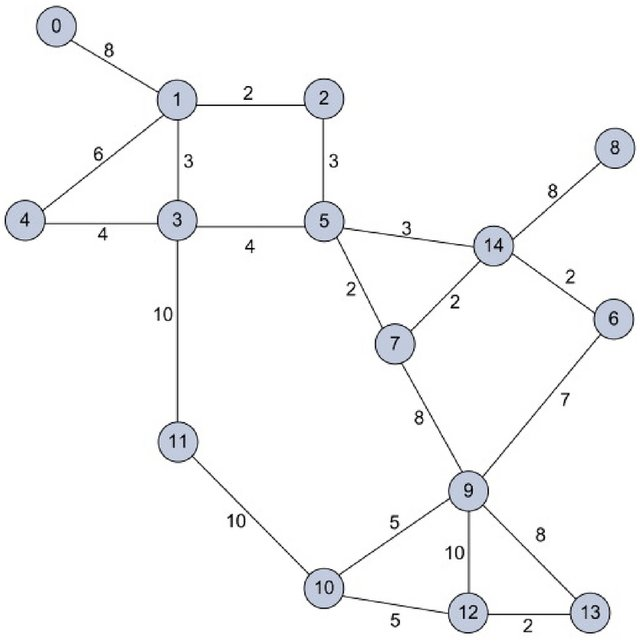
\includegraphics[width=0.45\textwidth]{Fig/Case-Study/Mandl/Mandl.png}
% \caption{Mandl’s benchmark network~\citep{mandl1980evaluation}.  
% The values displayed on each edge represent the baseline travel time between its two incident nodes, as provided in the original dataset.}
% \label{fig:mandl_network}
% \end{figure}
% % ------------------------- FIG
% Mandl’s Swiss network (see Fig.~\ref{fig:mandl_network}) is a small network consisting of 15 nodes and 21 links, initially used by~\cite{mandl1980evaluation} with a demand of 15,570 trips, and the demand is symmetric. This dataset is one of the few publicly accessible resources for the route planning problem and has emerged as the predominant benchmark instance. \rev{aa}{The predominant route length restriction confines each route to a maximum of 8 nodes. In this paper, we minimize human bias by permitting an unlimited number of nodes per route, thereby enabling the model to determine the optimal routes autonomously. These "unlimited" routes remain constrained by the condition that each node may be visited no more than once per route.}{For the sake of generality, different from~\cite{mandl1980evaluation}, we do not impose any restriction on the number of nodes per line.}

% --------------------------------------------------- 
% --------------------------------------------------- Appendix 4_alg+eval
% --------------------------------------------------- 
\section{Algorithmic Framework and Evaluation}
\label{sec:algorithmic-framework-and-evaluation}

\subsection{Parameter values for the proposed algorithm}
When computing adaptive network $\pazocal G_\text{PT}$ using the NSGA-III solution method described in the conference paper, we set the algorithmic parameters introduced therein as follows. 
The minimum path-overlap threshold is set to $J_{\text{min}}=0.5$, the crossover and mutation probabilities to $P_c=0.85$ and $P_m=0.35$, and the number of reference points to $N_{\text{ref}}=5^3=125$, respectively.

% ------------------------------------------------E.1
\subsection{Performance Metrics for Multi-Objective Optimization}\label{app:metrics}
We evaluate algorithm performance using three standard metrics for multi-objective optimization: Hypervolume (HV), Inverted Generational Distance (IGD), and Generational Distance (GD). 
%
The HV metric quantifies the volume of the objective space dominated by the Pareto solutions:
\begin{equation}
% \text{HV}(X, P) = \bigcup_{x \in X} v(x, P)
\text{HV}(X, P) = \Lambda \left( \bigcup_{x \in X} v(x, P) \right)
\end{equation}
where $X$ is the approximation set, $P$ is the reference point, and $v(x, P)$ is the hypervolume dominated by solution $x$ relative to $P$. Higher HV values indicate better coverage of the objective space. 
%
To ensure a fair comparison across algorithms, we report the HV metric calculated relative to a unified reference point. 
This reference point is constructed by collecting all solutions generated by all algorithms for each objective and selecting the worst (largest) value observed for each objective. 
% The same reference point is then used for all methods.
% Under this uniform evaluation standard, NSGA-III attains the largest HV$^\ast$, indicating the most favorable Pareto approximation among the compared methods.
%
The IGD metric measures the closeness of the approximation set to the true Pareto front:
\begin{equation}
\text{IGD}(X, \pazocal{P}^*) = \frac{\sum_{x^* \in \pazocal{P}^*} d(x^*, X)}{|\pazocal{P}^*|}
\end{equation}
where $\pazocal{P}^*$ is a set of reference points on the true Pareto front, $d(x^*, X)$ is the minimum distance from $x^*$ to any point in $X$, and $|\pazocal{P}^*|$ is the cardinality of $\pazocal{P}^*$. Lower IGD values indicate better convergence to the true Pareto front.
%
The GD metric complements IGD by measuring how far the obtained solutions are from the true Pareto front:
\begin{equation}
\text{GD}(X, \pazocal{P}^*) = \frac{\sum_{x \in X} d(x, \pazocal{P}^*)}{|X|}
\end{equation}
where $d(x, \pazocal{P}^*)$ is the minimum distance from a solution $x$ to the true Pareto front $\pazocal{P}^*$, and $|X|$ is the cardinality of the approximation set. Lower GD values indicate better convergence of the approximation set to the true Pareto front.
\rev{zg}{}{As the true Pareto front $\pazocal{P}^*$ is unknown for the instances considered, we approximate it, following standard practice in multi-objective optimization, by the non-dominated subset of the union of all solutions produced by all compared algorithms across all runs at a given variability level. The HV reference point is constructed analogously from the worst objective values observed across all algorithms (as described above), so that HV, IGD, and GD are all evaluated against a common, algorithm-agnostic reference.}



% ------------------------------------------------------
% % ++++++++++++++++++++ 6.1.1 - Static Network Optimization
% ------------------------------------------------------
% ------------------------------------------------E.1
\subsection{Implementation Details of the NSGA-III Environmental Selection}\label{A.Evolution}

% % ********************* 4.2.1
% \subsubsection{Crossover Operation}\label{sec:crossover}
% The crossover operation exchanges multiple PT lines between two parent solutions with probability $P_c$. The mechanism randomly selects a subset of line indices from each parent for exchange. Specifically, the number of lines to exchange is determined by $k = \text{random}(1, \min(|\pazocal{L}_1|, |\pazocal{L}_2|)/2)$, where $|\pazocal{L}_1|$ and $|\pazocal{L}_2|$ are the number of lines in parent 1 and parent 2, respectively. The algorithm then randomly samples $k$ line indices from each parent and exchanges the corresponding line configurations (including node sequences and vehicle allocations).

% The algorithm verifies network connectivity using depth-first search (Algorithm~\ref{alg:connectivity}) to ensure all OD pairs remain reachable after the exchange. For each OD pair $(o_k, d_k)$, the verification process ensures compliance with constraints~\eqref{st:12}-\eqref{st:13}.
% %
% If any OD pair becomes unreachable after the exchange, the crossover operation is deemed infeasible and the original parent solutions are retained unchanged. For valid offspring networks, vehicle allocation follows a two-stage process: each PT line receives one vehicle as baseline allocation ($n^\ell_{\text{base}} = 1$), then the remaining vehicles ($V_{\text{remaining}} = V_{\text{max}} - |\pazocal{L}|$) are distributed uniformly at random across all lines until the total fleet constraint~\eqref{st:10} is satisfied.

% % ===================== algDFS
% % \caption{DFS-based Network Connectivity Verification for OD Pairs}\label{alg:connectivity}
% % ===================== algDFSend

% % ********************* 4.2.2
% \subsubsection{Mutation Operation}\label{sec:mutation}
% Mutation perturbs a solution with probability $P_m$ by regenerating the path of a randomly selected PT line.
% For the chosen line $\ell$, the algorithm removes a contiguous segment of its node sequence and reconstructs it by iteratively selecting the next node from the set of unvisited neighbors $\pazocal{N}_{\text{unvisited}}(i)$ according to the probability rule in~\eqref{eq:node-addition-probability}.
% Each candidate node is checked for feasibility before being appended, ensuring that the regenerated subsequence forms a valid continuation of the line.
% %
% % Mutation creates new solutions with probability $P_m$ using controlled random path generation.\todoi{aa: It is not clear how new solutions are created. Be more concrete. Just saying ``using controlled path generation'' remains vague.}
% For constraints~\eqref{st:7}-\eqref{st:8}, the algorithm maintains a visited node registry and validates node additions against Miller-Tucker-Zemlin rules, tracking $u_i^\ell$ values to ensure constraint~\eqref{st:7} for each edge. To avoid generating networks that are too different from the existing ones, Jaccard similarity coefficients between candidate and existing line routes are computed, accepting only those with coefficients above a minimum threshold $J_{\text{min}}$. This prevents keeping solutions that are ``not interesting'', since they would have too high cost~$Z_3$~\eqref{eq:multi_objective}. Compliance with constraints~\eqref{st:12}-\eqref{st:13} is verified through connectivity checks using depth-first search.

% % ********************* 4.2.3
% \subsubsection{Reference Point-Based Selection}\label{sec:selection}

The algorithm adopts the reference-point-based environmental selection mechanism
of NSGA-III~\citep{deb2014nsga3} to maintain diversity across the three objectives in the conference paper.
Since all objectives are formulated as minimization problems, normalization is
performed on the combined population $R_t = P_t \cup Q_t$.
For each objective $j \in \{1,2,3\}$, objective-wise lower and upper bounds are
computed as
$z_j^{\min} = \min_{x \in R_t} Z_j(x)$ and
$z_j^{\max} = \max_{x \in R_t} Z_j(x)$,
and each objective is linearly scaled to $[0,1]$ accordingly.

A set of uniformly distributed reference points on the unit simplex is generated following the simplex-lattice design in~\cite{deb2014nsga3}.
% [Revision for aa: Which population? & No ellipses & Define Dominated]
As in standard multiobjective optimization, we say that solution $x$ dominates $y$ if $x$ is no worse than $y$ in all objectives and strictly better in at least one. We employ non-dominated sorting, which partitions the \textbf{combined population} $R_t = P_t \cup Q_t$ (comprising both parent and offspring individuals) into a sequence of Pareto fronts $F = \{F_1, F_2, \dots, F_l\}$.
% [Revision for aa: Exact list of partitions logic]
Here, $F_1$ contains the globally non-dominated solutions
% \footnote{A solution $x$ dominates $y$ if $x$ is no worse than $y$ in all objectives and strictly better in at least one.}
$F_2$ contains solutions dominated exclusively by members of $F_1$, and $F_l$ represents the \textit{critical front} where the cumulative count of solutions first meets or exceeds the population capacity $\textit{PopSize}$.
%
Each solution is associated with its nearest reference point by computing perpendicular distances from the solution to the reference lines in the normalized space. 
The environmental selection process adds complete Pareto fronts $F_1$ through $F_{l-1}$ sequentially; for the last front $F_l$, slots are filled by prioritizing solutions associated with reference points that have fewer assigned solutions to ensure diversity.


% ===================== algRepair
\begin{algorithm}[htbp]
\small
\caption{Feasibility-Oriented Path Completion for Line Repair}
\label{alg:bfs_repair}
\begin{algorithmic}[1]
    \renewcommand{\algorithmicrequire}{\textbf{Input:}}
    \renewcommand{\algorithmicensure}{\textbf{Output:}}
    
    \REQUIRE Substrate graph $\pazocal{G}=(\pazocal{N}, \pazocal{E})$, endpoints $(u, v)$, visited node set $\pazocal V_{\mathrm{used}}^\ell$
    \ENSURE Connecting path $\pazocal{P}_{u \to v}$ or $\emptyset$
    
    \STATE $\mathit{visited} \gets \{u\} \cup \pazocal V_{\mathrm{used}}^\ell$, $\mathit{queue} \gets \langle u \rangle$, $\mathit{parent}(\cdot) \gets \emptyset$
    
    \WHILE{$\mathit{queue}$ is not empty}
        \STATE $i \gets \mathit{queue}.\text{pop\_front}()$
        \IF{$i = v$}
            \STATE \textbf{break}
        \ENDIF
        \FOR{each neighbor $j$ of $i$ in $\pazocal{G}$}
            \IF{$j \notin \mathit{visited}$}
                \STATE $\mathit{visited} \gets \mathit{visited} \cup \{j\}$
                \STATE $\mathit{parent}(j) \gets i$
                \STATE $\mathit{queue}.\text{push\_back}(j)$
            \ENDIF
        \ENDFOR
    \ENDWHILE
    
    \IF{$v \notin \mathit{visited}$}
        \RETURN $\emptyset$
    \ENDIF
    \STATE $\pazocal{P}_{u \to v} \gets \text{Backtrack from } v \text{ to } u \text{ using } \mathit{parent}(\cdot)$
    \RETURN $\pazocal{P}_{u \to v}$
\end{algorithmic}
\end{algorithm}
% ===================== algRepairEnd

% ------------------------------------------------E.2
% \subsection{Performance of NSGA-III for Pareto-Front Generation}
%
% For generating Pareto fronts in our multi-objective optimization experiments, we employ NSGA-III
% , with NSGA-II serving as a benchmark to validate our algorithmic choice
% . 
%
% % ========================== SIDE-BY-SIDE TABLE (LEFT) AND FIGURE (RIGHT)
% \noindent
% \begin{minipage}[b]{0.45\textwidth}  % [t] -> [b]
% \centering
% \begin{threeparttable}
% \begin{small}
% \begin{tabular}{lrr}
% \toprule
% \textbf{Performance Metric} & \textbf{NSGA-II} & \textbf{NSGA-III} \\
% \midrule
% Hypervolume & 17.93 $\times 10^6$ & \textbf{40.73 $\times 10^6$} \\  
% Hypervolume Improvement  & - & \textbf{127.13} \\
% \midrule
% IGD (lower is better) & 0.088598 & \textbf{$<$ 0.001} \\
% IGD Change  & - & \textbf{$\approx$ -100.00} \\
% \midrule
% GD (lower is better) & 0.050887 & \textbf{$<$ 0.001} \\
% GD Change  & - & \textbf{$\approx$ -100.00} \\
% \midrule
% Common Ref. HV$^*$ & 41.22 $\times 10^6$ & \textbf{47.59 $\times 10^6$} \\
% Common HV Change  & - & \textbf{15.47} \\
% \bottomrule
% \end{tabular}
% \end{small}
% \begin{tablenotes}
% \footnotesize
% \item $^*$ The common–reference hypervolume evaluates all Pareto sets against a single fixed reference point, allowing an unbiased comparison across algorithms.
% \end{tablenotes}
% \end{threeparttable}
% \captionof{table}{Comparison of NSGA-II and NSGA-III Performance Metrics}
% \label{tab:algorithm_comparisonSELF}
% \end{minipage}%
% \hspace{0.05\textwidth}
% \begin{minipage}[b]{0.53\textwidth}  % [t] -> [b]
% \centering
% 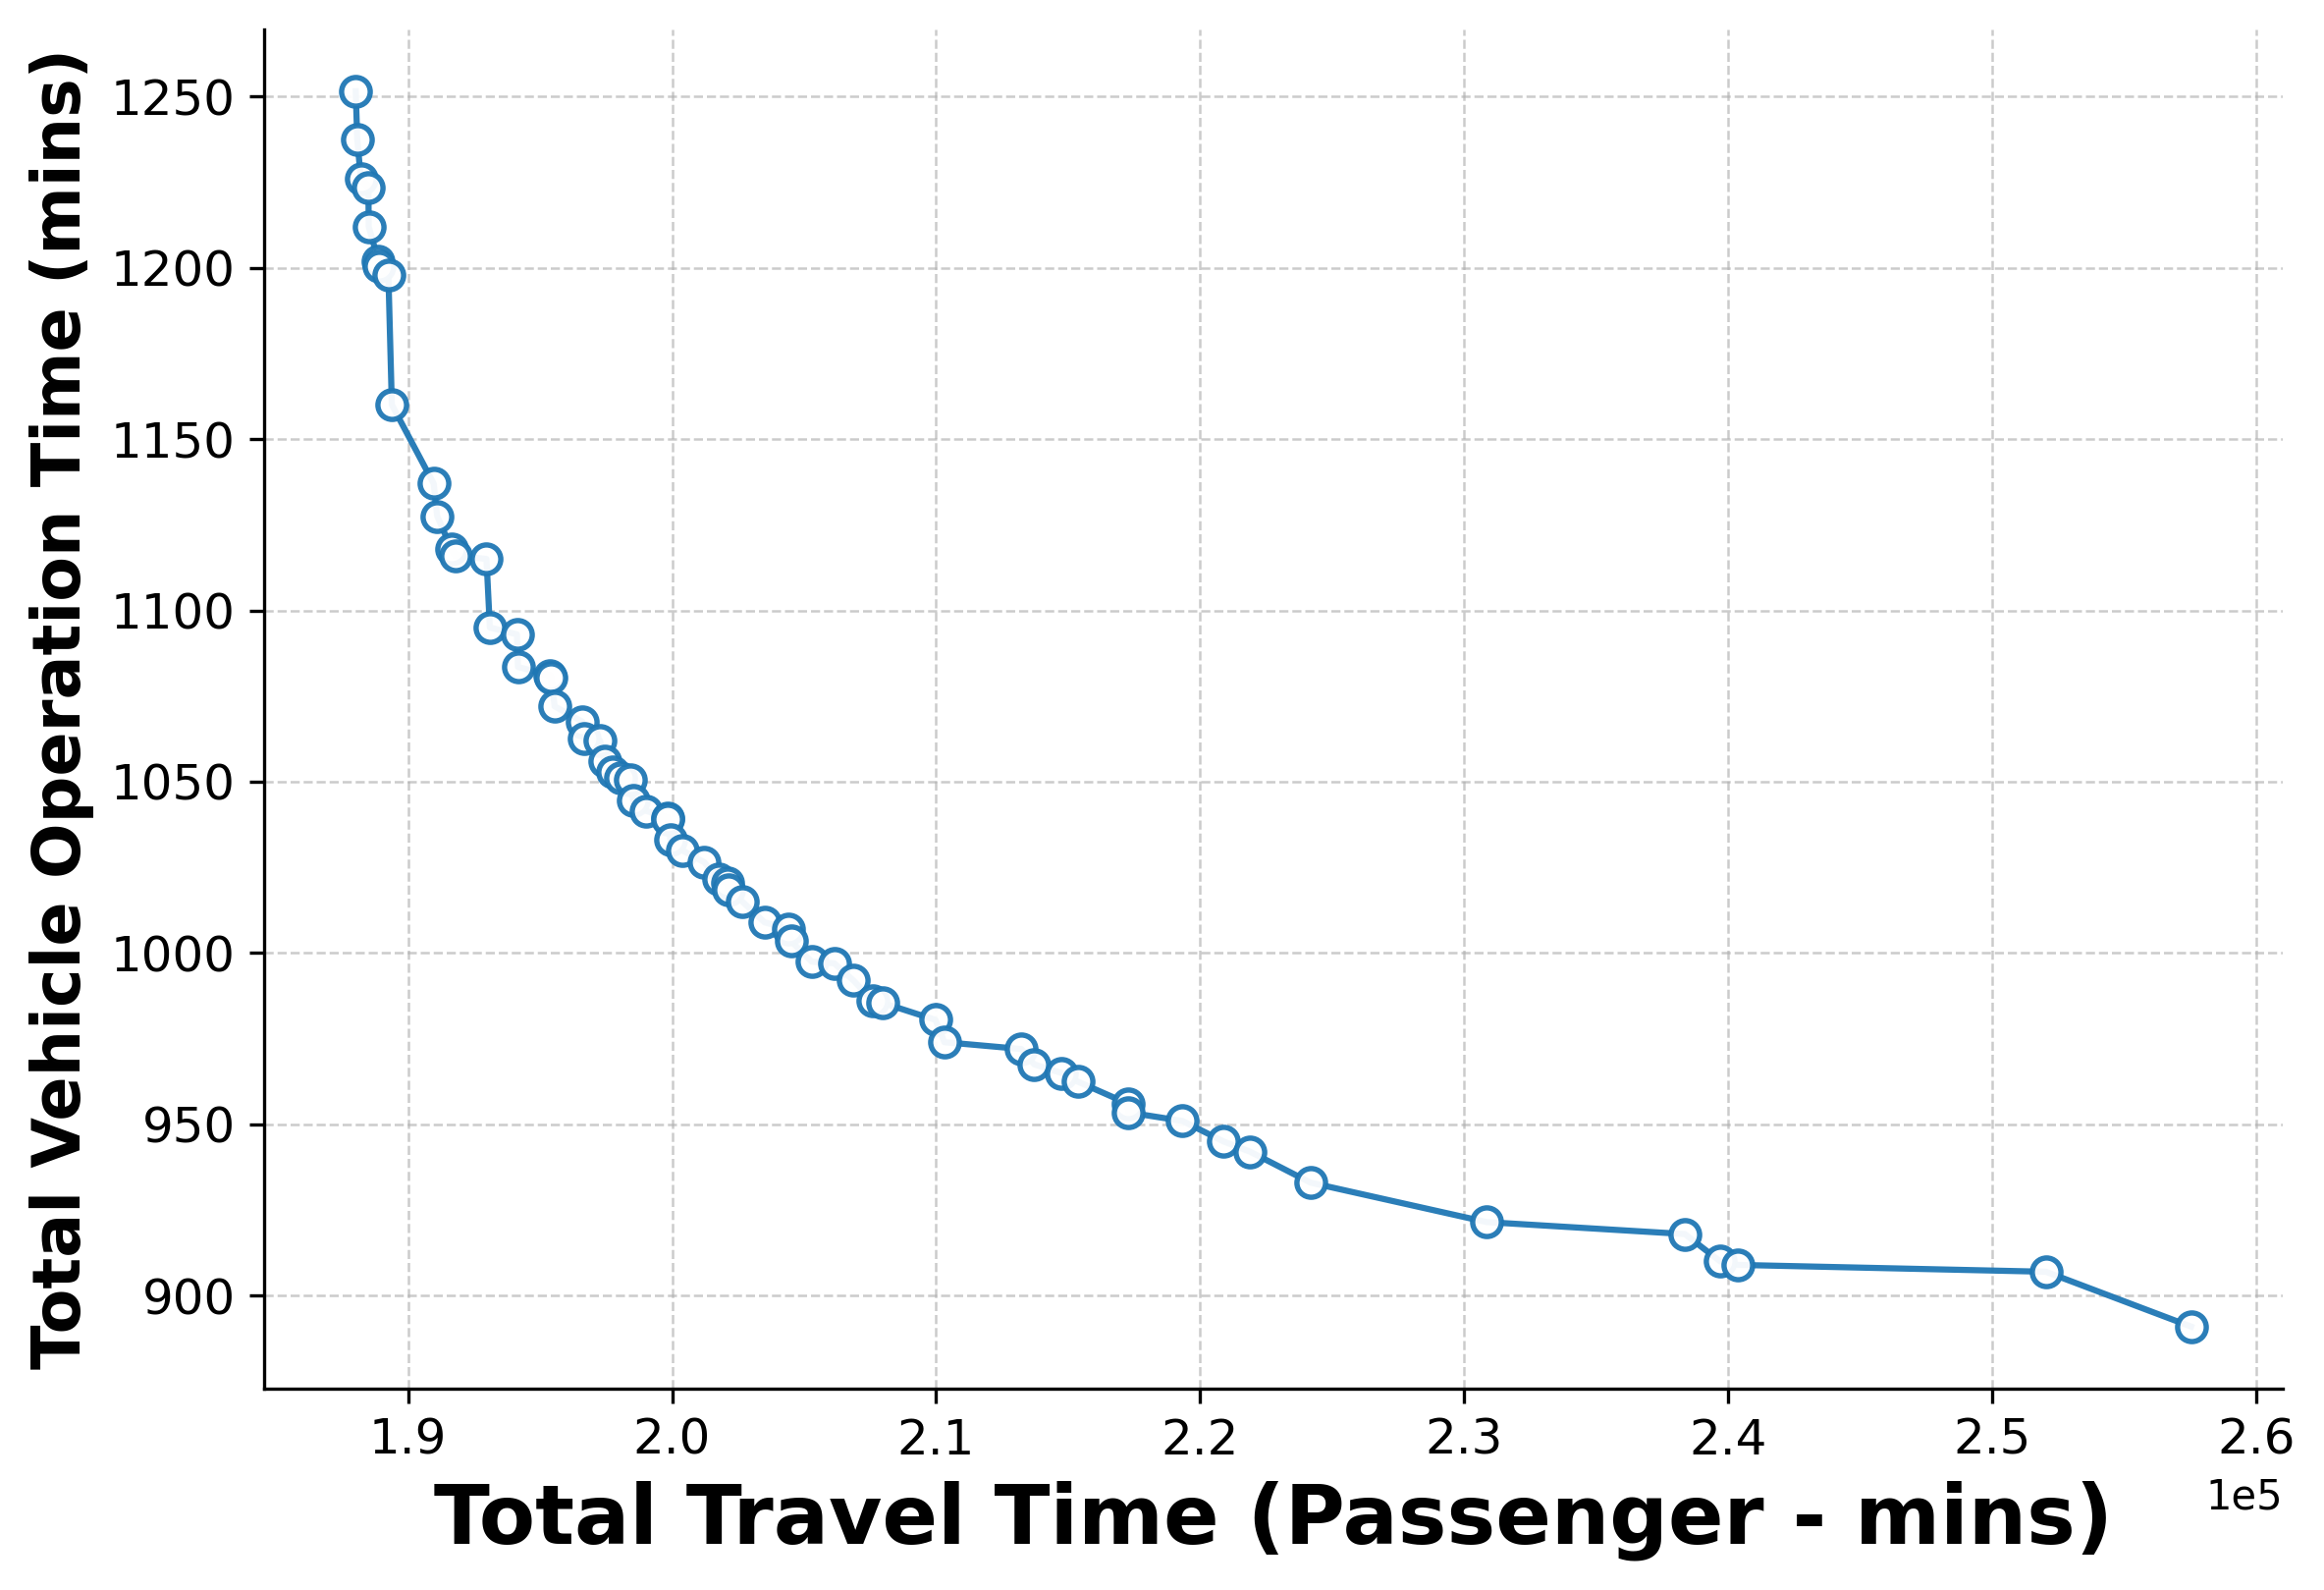
\includegraphics[width=\linewidth]{Fig/Analysis/C.4/nsga3_pareto_front_2d.png}
% \captionof{figure}{Pareto Frontier Generated by NSGA-III for Static Optimal Network}
% \label{fig:NSGA3SELF}
% \end{minipage}
% % ========================== END SIDE-BY-SIDE
%
% ========================== FIGURE ONLY
% \begin{figure}[htbp!]
% \centering
% 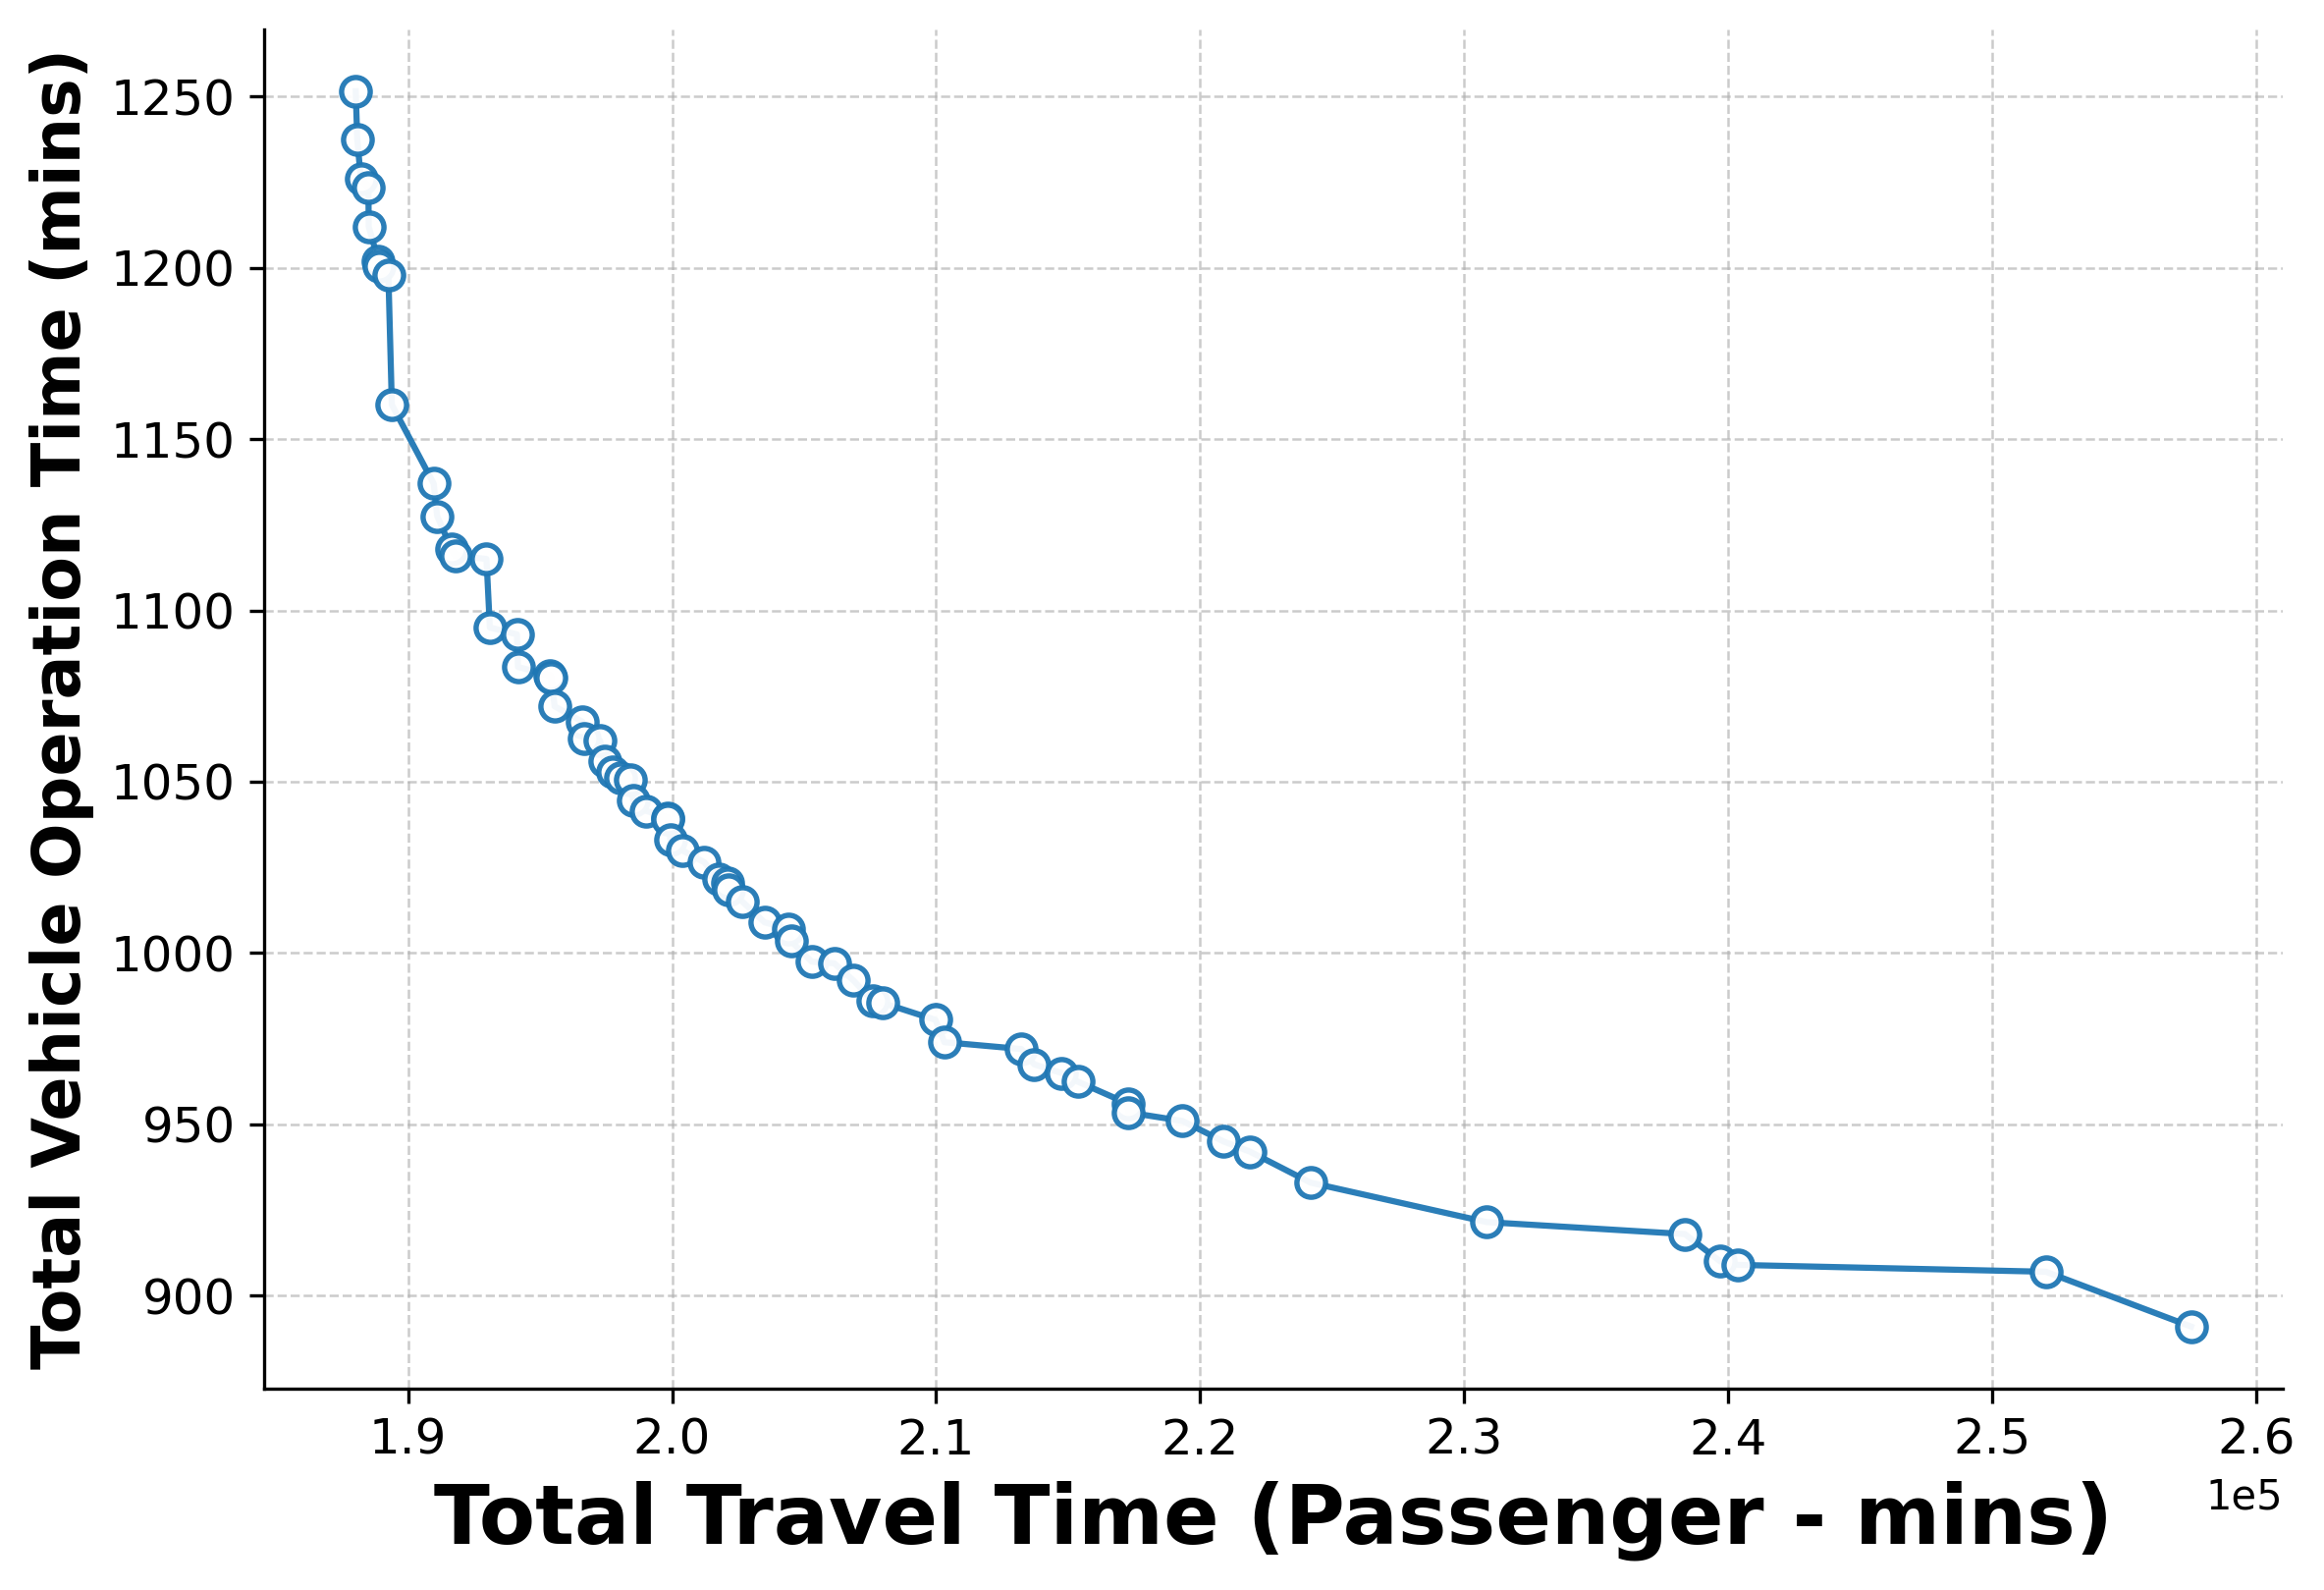
\includegraphics[width=0.65\linewidth]{Fig/Analysis/C.4/nsga3_pareto_front_2d.png}
% \caption{Pareto Frontier Generated by NSGA-III for Static Optimal Network}
% \label{fig:NSGA3SELF}
% \end{figure}
% ========================== END
%
% As shown in Table~\ref{tab:algorithm_comparisonSELF}, NSGA-III significantly outperforms NSGA-II across all metrics. 
% The static optimal-network experiment in Fig.~\ref{fig:NSGA3SELF} is generated by jointly optimizing passenger travel time ($Z_1$) and operational cost ($Z_2$) via our solution method (\S~\ref{sec:problemStatement}) without adaptive mechanisms; therefore, the network is static.
% Fig.~\ref{fig:NSGA3SELF} displays the resulting Pareto frontier with non-dominated solutions balancing vehicle operation time against passenger travel time. 
% %
% We identify the representative static solution as the solution that is closest to the ideal point, 
% defined as the point where all objectives attain their minimum value. 
% Specifically, we select the Pareto-optimal solution that minimizes the normalized Euclidean distance 
% to this ideal point. 
% This choice corresponds to the “knee’’ region of the Pareto frontier, where any further improvement 
% in one objective would cause a disproportionately large deterioration in the other.

% ------------------------------------------------------ 
% % ++++++++++++++++++++ 6.1 - Algorithm Performance Analysis 
% ------------------------------------------------------
\subsection{Algorithm Performance Evaluation}

Algorithmic performance is evaluated via 
the Hypervolume (HV), the Inverted Generational Distance (IGD), and the Generational Distance (GD), which are standard performance metrics in multi-objective evolutionary optimization
as surveyed in~\citep{riquelme2015performance}.\footnote{Formal definitions and computational details are provided in App.~\ref{app:metrics}.}
The Hypervolume (HV) evaluates both convergence and diversity by measuring the dominated volume in the objective space, where higher values indicate better performance ($\uparrow$). In contrast, GD and IGD are distance-based indicators that assess convergence to a reference Pareto front, with lower values indicating better convergence ($\downarrow$).


To evaluate the effectiveness of NSGA-III for \rev{zg}{real-time}{forecast-triggered} PT redesign, we compare it with NSGA-II~\citep{deb2002fast} and hybrid multi-objective algorithms that combine non-dominated sorting with variable neighborhood descent, based on Mandl’s Swiss network.
Specifically, we consider two Non-dominated Sorting Variable Neighborhood Descent (NSVND) variants inspired by the integration of NSGA-II with variable neighborhood search strategies~\citep{hansen2001variable}.
The first variant (NSVND-II) follows the NSGA-II framework while replacing crossover and mutation with variable neighborhood descent, whereas the second variant (NSVND-III) further incorporates an adaptive neighborhood selection mechanism to enhance exploration of the Pareto frontier.

% ========================== tableHVIGD©
\begin{table}[htbp]
\centering
\footnotesize
\setlength{\tabcolsep}{4.5pt}
\renewcommand{\arraystretch}{1.15}
\begin{threeparttable}
\begin{tabular}{@{}l*{4}{c}@{}}
\toprule
\textbf{Performance Metric} & \textbf{NSGA-II} & \textbf{NSGA-III} & \textbf{NSVND-II} & \textbf{NSVND-III} \\
% \midrule
% Hypervolume (HV, higher is better) 
% & $3.71\times10^9$ 
% & $7.09\times10^9$ 
% & $7.28\times10^9$ 
% & \textbf{$7.36\times10^9$} \\
% HV Improvement (\%)\tnote{a} 
% & -- 
% & 91.01 
% & 96.23 
% & \textbf{98.38} \\
\midrule
Inverted Generational Distance (IGD, lower is better) 
& 347.64 
& \textbf{22.63} 
& 38.90 
& 34.80 \\
IGD Change\tnote{a} 
& -- 
& \textbf{-325.01} 
& -308.74 
& -312.84 \\
\midrule
Generational Distance (GD, lower is better) 
& 75.36 
& \textbf{17.17} 
& 24.40 
& 22.80 \\
GD Change\tnote{a} 
& -- 
& \textbf{-58.19} 
& -50.96 
& -52.56 \\
\midrule
Hypervolume (HV, higher is better) \tnote{b} 
& $30.52\times10^9$ 
& \textbf{$31.49\times10^9$} 
& $31.23\times10^9$ 
& $31.31\times10^9$ \\
HV Change\tnote{a} 
& -- 
& \textbf{0.97$\times10^9$} 
& 0.71$\times10^9$ 
& 0.79$\times10^9$ \\
\bottomrule
\end{tabular}

\begin{tablenotes}\footnotesize
\item[a] Improvement/Change are computed relative to NSGA-II (baseline).
\item[b] HV uses a single fixed reference point shared by all algorithms.
\end{tablenotes}
\end{threeparttable}
\caption{Multi-objective algorithm comparison under noise-free travel times ($cv=0$).}
\label{tab:algorithm_comparison_simple}
\end{table}
% ========================== tableHVIGDEND

Table~\ref{tab:algorithm_comparison_simple} presents an algorithm performance comparison for adaptive network optimization assuming no travel time deviation from the nominal ones (\textit{cv}=0).
% ~\footnote{
Although no adaptive redesign is required when $cv=0$, this setting provides a noise–free benchmark for comparing optimization algorithms.
% } 
% While NSVND-series algorithms demonstrate superior hypervolume metrics, they exhibit significantly inferior convergence as evidenced by their poor IGD and GD values. In contrast, 
NSGA-III maintains an optimal balance between solution diversity (high hypervolume) and convergence precision.
%
% To enable a fair cross-algorithm comparison, we additionally report the hypervolume computed with a common fixed reference point (HV$^\ast$).%
% \footnote{The common reference point is constructed by first collecting all solutions generated by all algorithms and then taking, for each objective, the worst (largest) value observed. This single reference point is shared by all algorithms, enabling their hypervolume values to be directly comparable.}
% Under this uniform evaluation standard, NSGA-III attains the largest HV$^\ast$, indicating the most favorable Pareto approximation among the compared methods.


\section{Network Performance Metrics}\label{A.PerformanceMetrics}

This appendix details the performance indicators used in the experiments.

For each realization $\omega \in \Omega$ of stochastic travel times, we define the following performance metrics: \textbf{20\% Improvement Share (IS$_{20}$)}, \textbf{Operational Cost Reduction (OCR)}, and \textbf{Line Overlap (LO)}. Since these metrics vary with the realized scenario $\omega$, they are treated as random variables. In our numerical results, we report their empirical averages (and standard deviations) over 30 independent realizations.

\begin{itemize}
    \item \textbf{20\% improv. share (\%):} The proportion of OD pairs experiencing a travel time reduction of at least 20\% under realization $\omega$.
    \begin{align}
        \label{eq:metricIS20}
        \text{IS$_{20}$}(\omega) = \frac{\sum_{k \in \pazocal{K}} \mathbb{I} \left( \frac{t_k^0 - t_k^*(\omega)}{t_k^0} \geq 20\% \right)}{|\pazocal{K}|} \times 100\%, \text{ where } \mathbb{I}(\cdot) \text{ is the indicator function.}
    \end{align}
    Here $t_k^0$ and $t_k^*(\omega)$ denote the original and adaptive travel times for OD pair $k$, respectively. Since both depend on random travel-time realizations, $\text{IS$_{20}$}$ is a random variable.

    \item \textbf{Operational Cost Reduction (OCR)}
\begin{equation}
\label{eq:metricOCR}
\operatorname{OCR}(\omega)
=
\frac{
    \sum_{\ell \in \pazocal{L}} n^\ell t^\ell
    -
    \sum_{\ell \in \pazocal{L}} n^{\ell,*}(\omega) t^{\ell,*}(\omega)
}{
    \sum_{\ell \in \pazocal{L}} n^\ell t^\ell
}
\times 100\%.
\end{equation}
    Here $t^\ell$ and $t^{\ell,*}(\omega)$ are the realized travel times of line $\ell$ in the original and adaptive networks, respectively,
    and $n^\ell$ and $n^{\ell,*}$ are the corresponding vehicle allocations.
    Because $t^\ell$ and $t^{\ell,*}(\omega)$ vary with the realization, OCR is also a random variable.

    \item \textbf{Line Overlap (LO)}
    To quantify structural similarity between the original and adaptive networks, we use the Jaccard index:
\begin{equation}
\label{eq:metricRO}
\operatorname{LO}(\omega)
=
\frac{
    \left| \pazocal{E}_{\mathrm{PT}}
    \cap
    \pazocal{E}_{\mathrm{PT}}^{*}(\omega) \right|
}{
    \left| \pazocal{E}_{\mathrm{PT}}
    \cup
    \pazocal{E}_{\mathrm{PT}}^{*}(\omega) \right|
}
\times 100\%.
\end{equation}
    Here $\pazocal{E}_{\mathrm{PT}}$ and $\pazocal{E}_{\mathrm{PT}}^*(\omega)$ denote the realized edge sets of the original and adaptive networks, respectively.
    Since these sets depend on the travel-time realization, LO is likewise a random variable.

\end{itemize}

The numerical results therefore report the \emph{empirical means} $\pm$ \emph{standard deviations} of IS$_{20}$, OCR, and LO over the 30 realizations $\omega \in \Omega$, providing a stochastic assessment of adaptive-network performance.

% -------------- App.D.1
\subsection{Forecast-error Sensitivity Analysis}
\label{app:forecastValue}

This appendix provides the formal basis and the full results for the forecast-error sensitivity analysis summarized in the main text. App.~\ref{app:forecastValueMetrics} defines the two hypervolume-based summaries used to quantify \rev{aa}{}{the impact of the} forecast \rev{aa}{value}{error in the optimization output} (the \emph{forecast-value headroom} and the \emph{forecast value retained}). App.~\ref{app:forecast_sensitivity} then applies these metrics to the Mandl instance and reports the detailed results across variability levels and error scales~$\alpha$.

We deliberately grade the entire front rather than any single selected design: the optimizer returns a set of non-dominated trade-offs, and the specific compromise that gets deployed (e.g., the selected compromise solution in the conference paper) is chosen by the operator after the front is produced, according to priorities the algorithm itself does not fix. Tying the sensitivity analysis to one such pre-selected point would conflate two different effects — forecast quality and the arbitrary choice of operating point — since the operator could simply pick a different point on the front to offset a degraded solution, masking a genuine impact of the forecast accuracy on the quality of the solutions (or manufacturing a spurious one). Hypervolume sidesteps this confound by scoring the whole menu of options the operator has to choose from in a single scalar: a drop in $HV$ reflects an actual shrinkage of what is available to the operator, not an artifact of which point happens to be selected.

\subsubsection{Forecast-value metrics}
\label{app:forecastValueMetrics}

We quantify whether the forecast helps the redesign, and by how much. Holding the realized \rev{aa}{scenario}{link travel times} $\{t_{ij}^{\omega}\}$ fixed, we vary \emph{only} the forecast link times $\hat{t}_{ij}^{\omega}(\alpha)$ handed to the optimizer ($\hat t_{ij}^{\omega}(\alpha)=t_{ij}^{\omega}\exp(\alpha\eta_{ij}^{\omega})$) and score the returned Pareto front on the true realized times $t_{ij}^{\omega}$. Since only the error scale $\alpha$ changes, any difference is attributable to forecast quality alone. Each front is graded by its hypervolume $HV$, the volume it dominates in the space of the three performance metrics $(\mathrm{IS}_{20},\mathrm{OCR},\mathrm{LO})$ defined in Appendix~
ef{A.PerformanceMetrics}, measured from the single fixed reference point of App.~\ref{app:metrics}; a larger $HV$ is better\rev{aa}{ and needs no weighting of the three metrics}{}. For each seed $s\in\{1,\dots,S\}$ (with $S=30$ random seeds) and each variability level $\textit{cv}$ we compute three fronts:
\begin{itemize}
    \item \emph{No forecast}: \rev{aa}{}{the optimizer uses the} nominal link times $t_{ij}^{0}$\rev{aa}{, giving the \emph{floor}}{We call the corresponding hypervolume} $HV^{\mathrm{NF}}_{s,\textit{cv}}$ \rev{aa}{(lower bound)}{\emph{floor}, since it corresponds to the lower bound}.

    \item \emph{Perfect foresight} ($\alpha=0$): the optimizer uses the true realized times $t_{ij}^{\omega}=\hat{t}_{ij}^{\omega}(0)$. We denote the corresponding hypervolume by $HV^{\mathrm{PF}}_{s,\textit{cv}}\equiv HV_{s,\textit{cv},0}$ and call it the \emph{ceiling}, since it represents the upper bound.

    \item \emph{Error-$\alpha$ forecast}: the forecast $\hat{t}_{ij}^{\omega}(\alpha)$ defined above ($\alpha=1$ the empirical DCRNN level, $\alpha>1$ a stress test), giving the intermediate hypervolume $HV_{s,\textit{cv},\alpha}$.
\end{itemize}
Because a seed fixes both the realized scenario and the sampled errors $\eta$, each $HV_{s,\textit{cv},\alpha}$ is a single realization, and all reported 95\% confidence intervals reflect variation across the $S$ seeds. We measure the climb from floor to ceiling in two steps.

\paragraph{Step 1: is there anything to gain?} The \emph{forecast-value headroom} $H_{s,\textit{cv}}=\bigl(HV^{\mathrm{PF}}_{s,\textit{cv}}-HV^{\mathrm{NF}}_{s,\textit{cv}}\bigr)/HV^{\mathrm{PF}}_{s,\textit{cv}}$ is the floor-to-ceiling gap as a fraction of the ceiling: $H\approx0$ means even a perfect forecast barely beats nominal times, whereas a large $H$ signals real value to capture. We report the mean $\bar H_c$ across seeds with a 95\% confidence interval.

\paragraph{Step 2: how much do we actually capture?} The \emph{forecast value retained} $R_{s,\textit{cv},\alpha}=\bigl(HV_{s,\textit{cv},\alpha}-HV^{\mathrm{NF}}_{s,\textit{cv}}\bigr)/\bigl(HV^{\mathrm{PF}}_{s,\textit{cv}}-HV^{\mathrm{NF}}_{s,\textit{cv}}\bigr)$ places an error-$\alpha$ forecast on that same scale: $R=1$ matches perfect foresight, $R=0$ matches no forecast, and $R<0$ is worse than no forecast. Since this gap can be tiny for a single seed (making per-seed ratios erratic, unlike $H_{s,\textit{cv}}$, whose denominator $HV^{\mathrm{PF}}_{s,\textit{cv}}$ stays bounded away from zero), we aggregate it as a ratio of averages,
\begin{equation}
\bar R_{c,\alpha}=\frac{\tfrac1S\sum_s\big(HV_{s,\textit{cv},\alpha}-HV^{\mathrm{NF}}_{s,\textit{cv}}\big)}{\tfrac1S\sum_s\big(HV^{\mathrm{PF}}_{s,\textit{cv}}-HV^{\mathrm{NF}}_{s,\textit{cv}}\big)},
\end{equation}
with a 95\% confidence interval and $\bar R_{c,0}=1$ by construction. At the lowest variability ($cv=0.05$) the floor and ceiling are statistically indistinguishable (Fig.~\ref{fig:forecast_headroom}), so $R$ is undefined and we omit this level from Fig.~\ref{fig:forecast_retained}.

\subsubsection{\rev{zg}{}{Forecast-value results}}\label{app:forecast_sensitivity}

Fig.~\ref{fig:forecast_value_hv} reports the forecast-value metrics of App.~\ref{app:forecastValueMetrics} for the 4-line Mandl instance. By construction, these metrics separate two otherwise-conflated effects: the redesign opportunity created by travel-time variability (the \emph{headroom}), and the accuracy with which the forecast exploits it (the \emph{retained value}). Fig.~\ref{fig:forecast_value_hv}(a) shows that the headroom is negligible at $cv=0.05$ and grows with variability, reaching roughly half of the perfect-foresight hypervolume at $cv=1.0$: a forecast is valuable primarily when variability creates a genuine redesign opportunity, whereas in stable conditions even an oracle adds little because the nominal times $t_{ij}^{0}$ already describe the operating state. Fig.~\ref{fig:forecast_value_hv}(b) shows that the empirical forecast ($\alpha=1$) retains essentially all of this available value, and moderate amplification ($\alpha=1.5$) causes no visible collapse, consistent with the intended robustness claim. \textbf{The method's gains are therefore driven mainly by the redesign opportunities that variability creates, not by a dependence on high-precision forecasts.}

% -------------------------- Figure: Forecast-value headroom + retained
\begin{center}
\captionsetup{type=figure}
\centering
\begin{subfigure}[t]{0.49\textwidth}
\centering
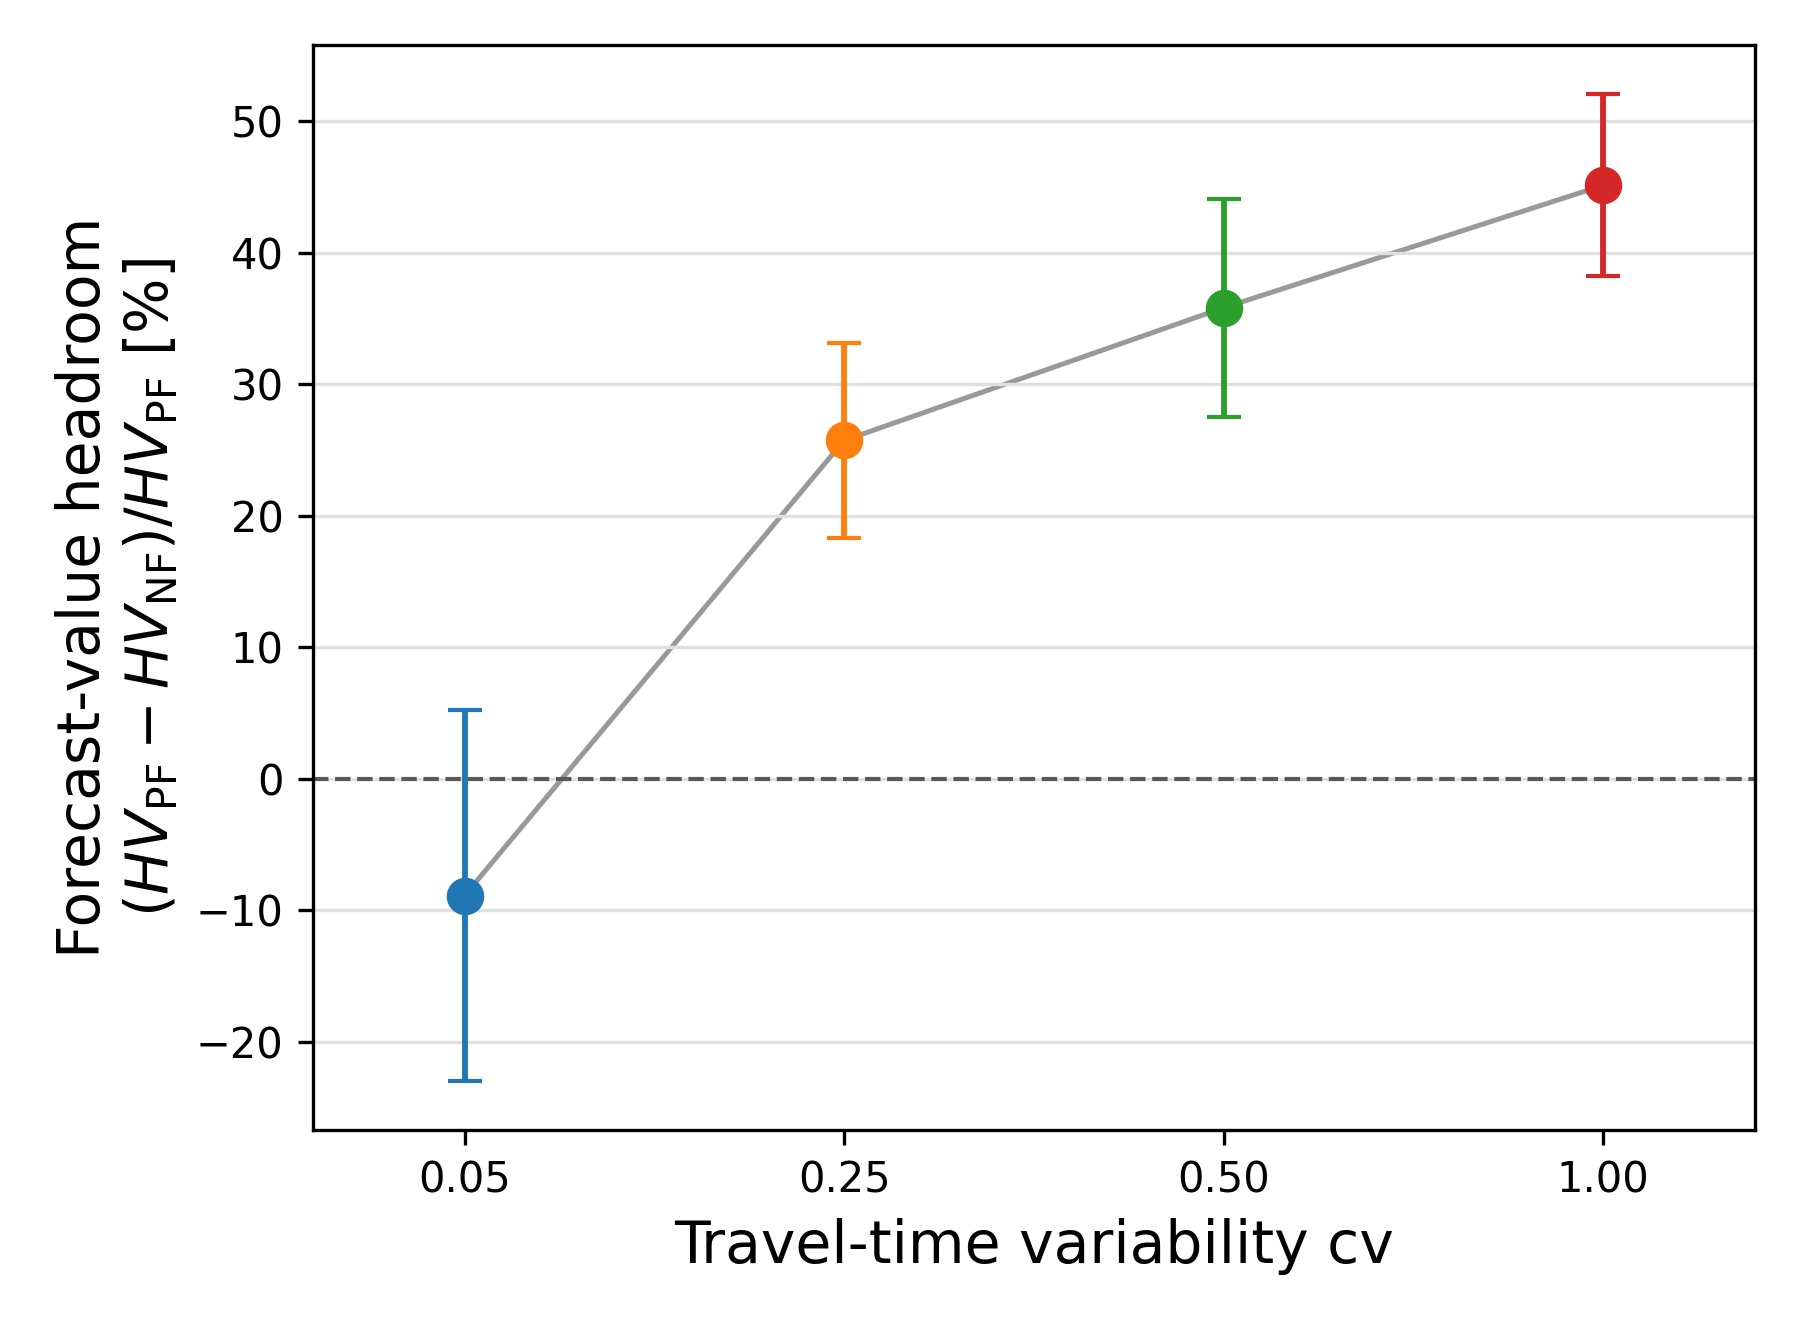
\includegraphics[width=\textwidth]{Fig/Analysis/6.2.2/forecast_headroom_by_cv.png}
\caption{\rev{zg}{}{\textbf{Forecast-value headroom $\bar H_c$ vs.\ $cv$} (mean over 30 seeds; 95\% CI bars). Headroom is the share of the perfect-foresight hypervolume attributable to using any forecast.}}
\label{fig:forecast_headroom}
\end{subfigure}
\hfill
\begin{subfigure}[t]{0.49\textwidth}
\centering
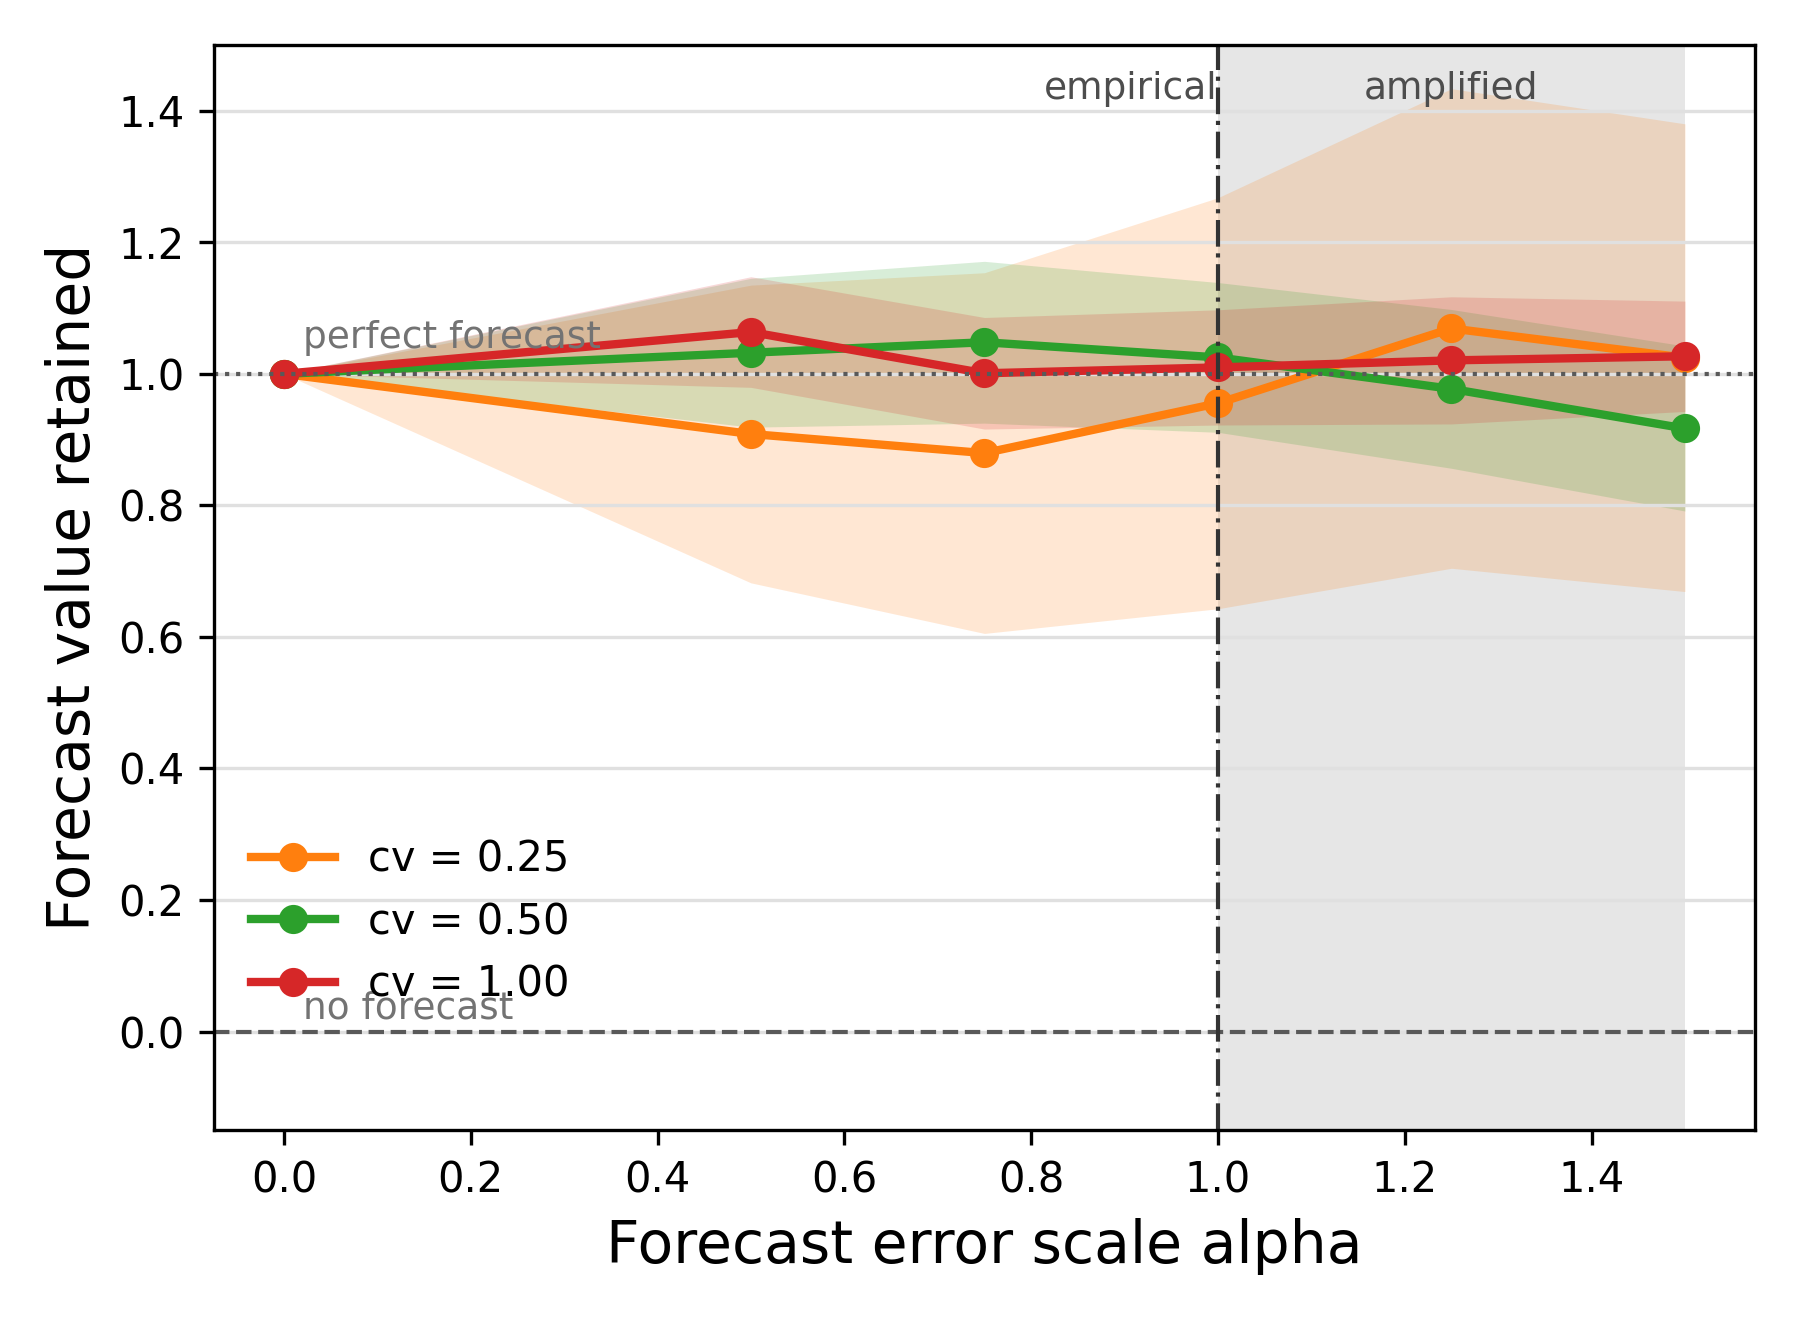
\includegraphics[width=\textwidth]{Fig/Analysis/6.2.2/forecast_value_retained_hypervolume.png}
\caption{\rev{zg}{}{\textbf{Forecast value retained $\bar R_{c,\alpha}$ vs.\ error scale $\alpha$} (ratio-of-means; shaded 95\% CI). $\alpha=1$ is the empirical DCRNN error; $\alpha>1$ is a stress test.}}
\label{fig:forecast_retained}
\end{subfigure}
\caption{\rev{zg}{}{Hypervolume-based forecast value on the Mandl redesign (mean over 30 seeds): (a) headroom available from any forecast as variability grows; (b) fraction of headroom retained as forecast error is amplified. The method retains essentially all available value at the empirical error level and degrades only under severe amplification.}}
\label{fig:forecast_value_hv}
\end{center}

\subsection{\rev{zg}{}{Exceedance Probability of OD-Level Improvement Rates by Bus-Line Quantity}}\label{App:D3_ImprovementICDF}

\rev{aa}{}{For each variability level \(\textit{cv}=0.05, 0.25, 0.5, 1\) and each random seed \(\omega \in \Omega\), we compute the empirical complementary cumulative distribution function (CCDF) of the percentage travel-time improvement over the set of OD pairs. Thus, for a threshold \(x\), the CCDF gives the fraction of OD pairs whose percentage improvement is larger than \(x\). The solid lines in Fig.~\ref{fig:appendix_improvement_exceedance_all_routes}  report the pointwise average of these empirical CCDFs over the 30 seeds.
The figure shows that proactive redesign becomes beneficial only under large travel-time variability, namely for ($cv \geq 0.5$). For lower variability levels, it worsens travel times for a larger fraction of OD pairs than it improves.
}


\rev{aa}{Fig.~\ref{fig:appendix_improvement_exceedance_all_routes} reports the trimmed-mean exceedance curves of OD-level improvement rates. For each seed $\omega$, the OD-level improvement rates are first sorted to form a per-seed quantile curve $Q_\omega(p)$, where $p$ denotes the exceedance probability. The extreme seed curves are then removed and the remaining per-seed quantile curves are averaged pointwise. Thus, the plotted line is a trimmed mean of per-seed quantile curves, rather than a curve computed from pooled OD pairs across all seeds. Across line quantities, the curves make it possible to compare both the intensity of improvements and the share of OD pairs receiving a given minimum percentage reduction under different variability levels.}{}

\begin{center}
\captionsetup{type=figure}
    \centering
    \begin{subfigure}[t]{0.47\textwidth}
        \centering
        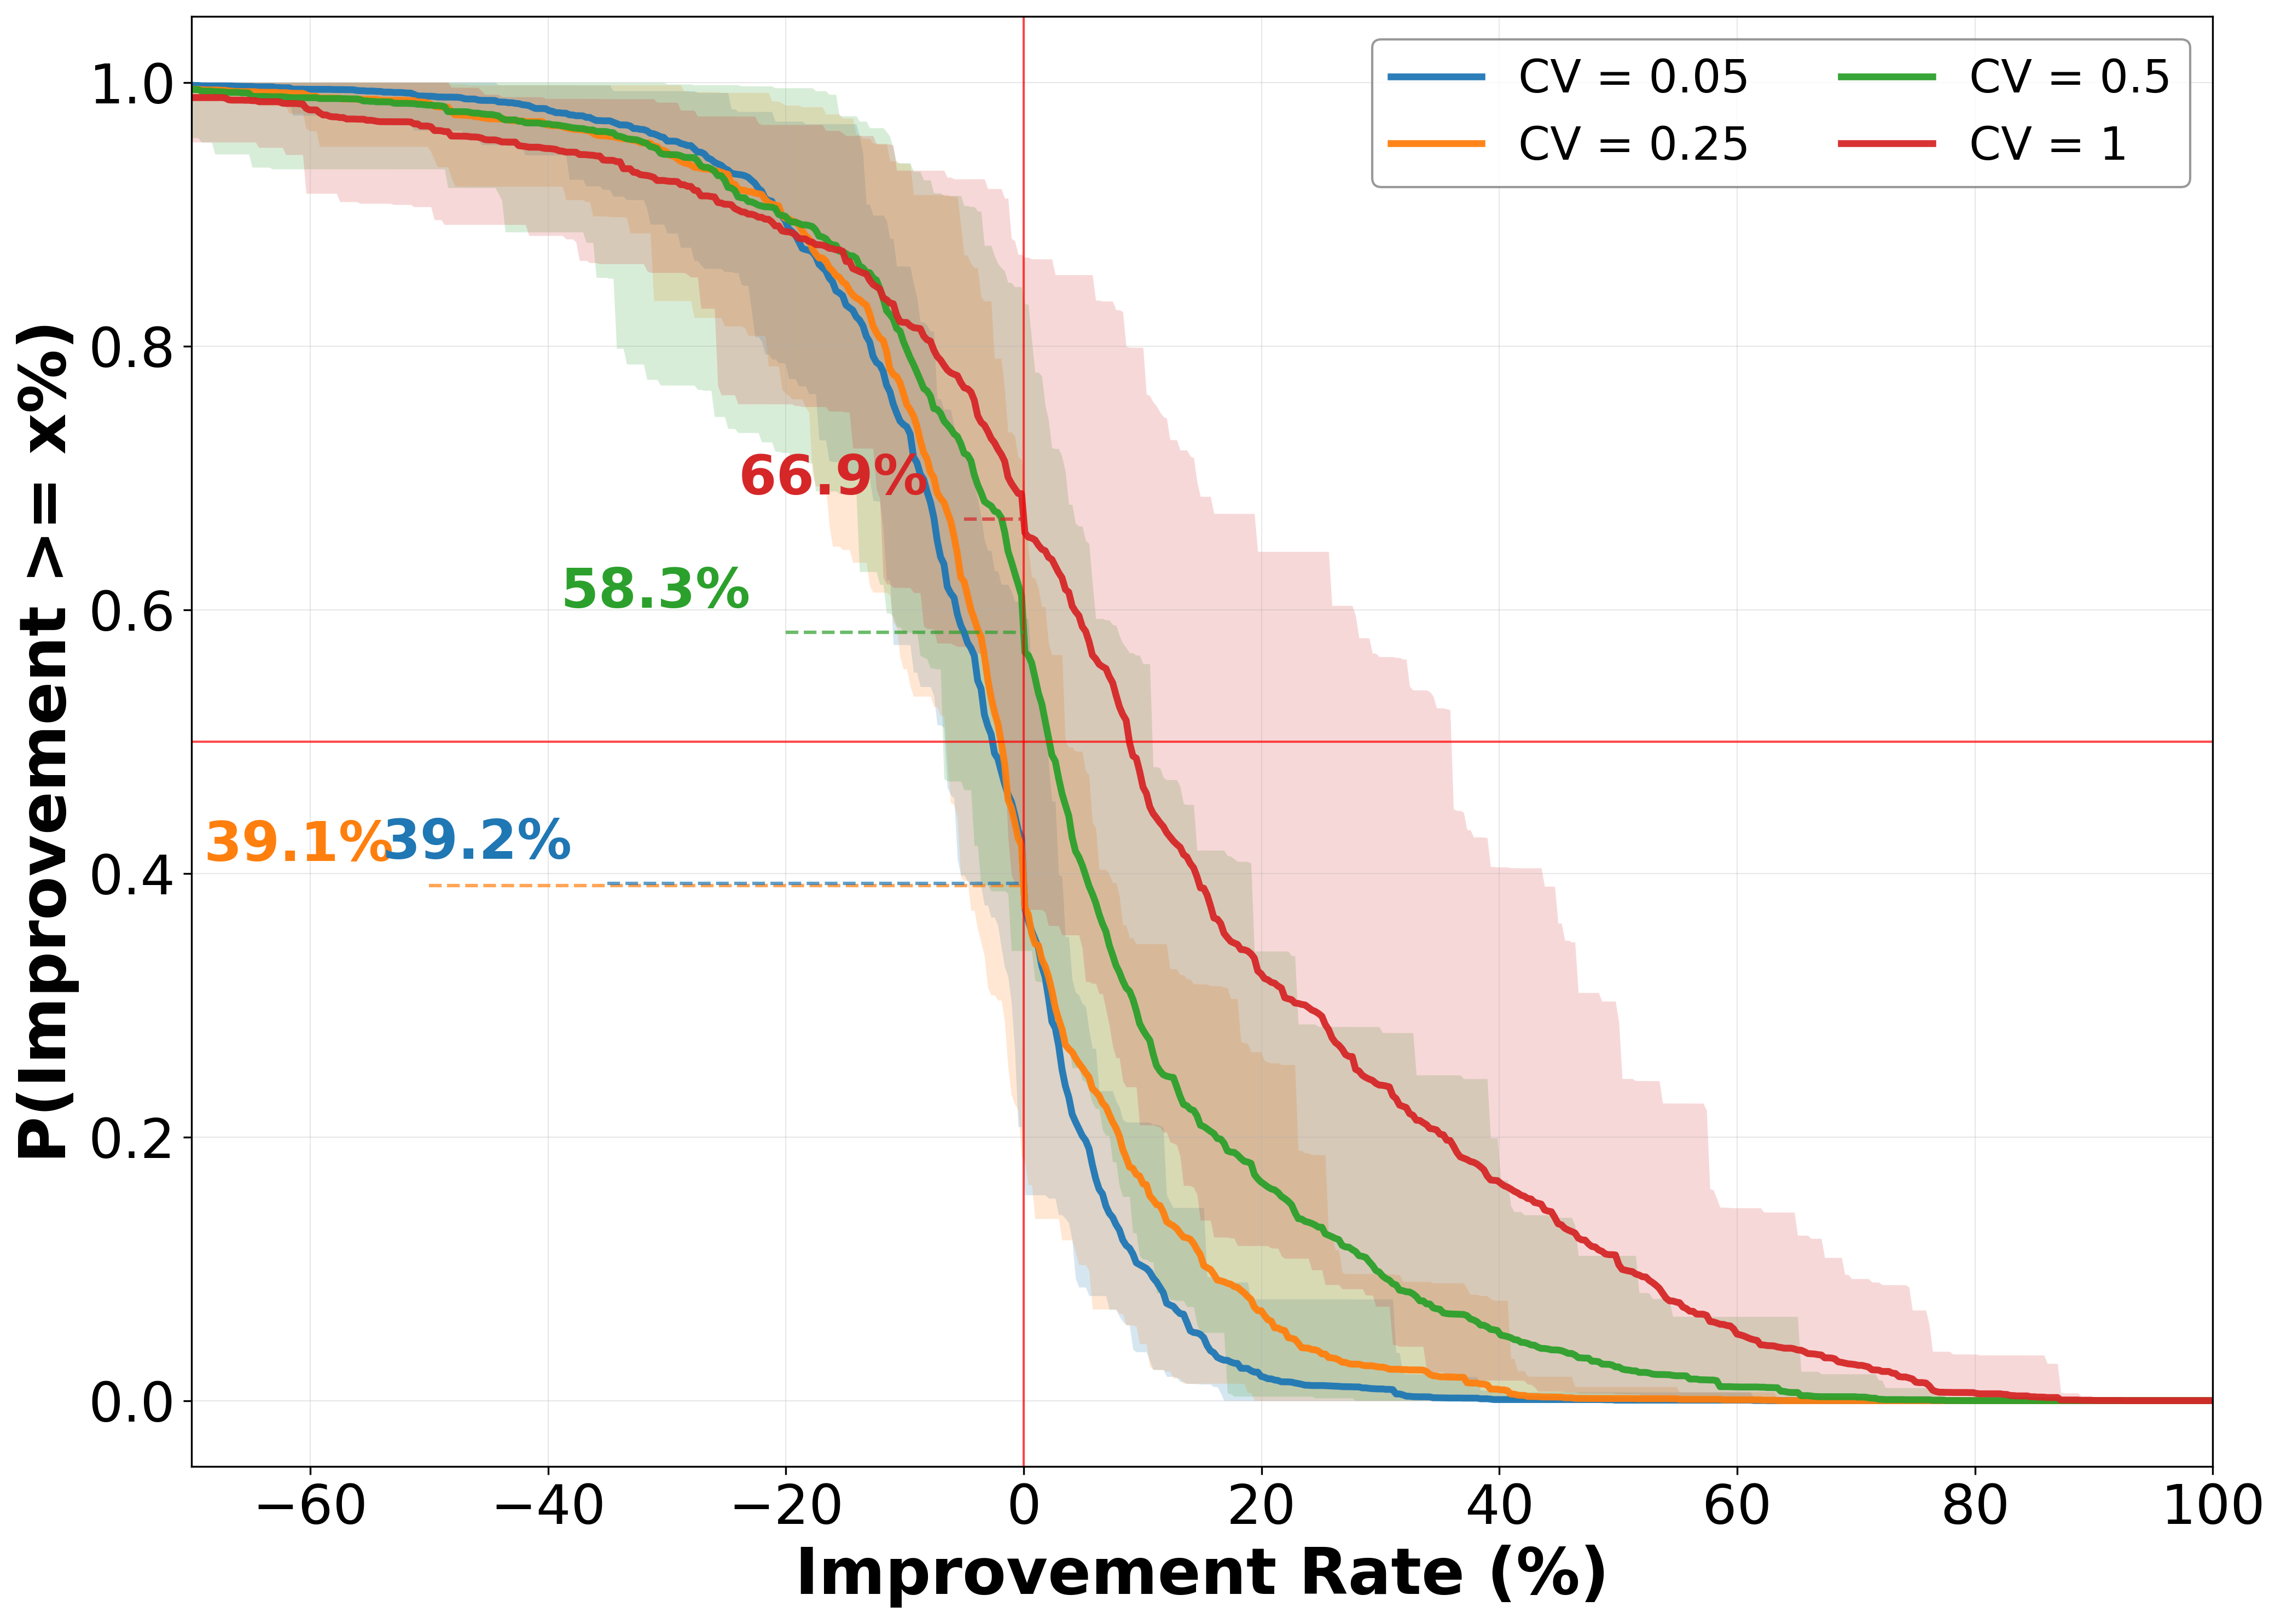
\includegraphics[width=\textwidth]{Fig/Analysis/D.1/improvement_icdf_4routes_all_cvs_trimmed_range.png}
        \caption{4 lines}
        \label{fig:appendix_improvement_exceedance_4routes}
    \end{subfigure}
    \hfill
    \begin{subfigure}[t]{0.47\textwidth}
        \centering
        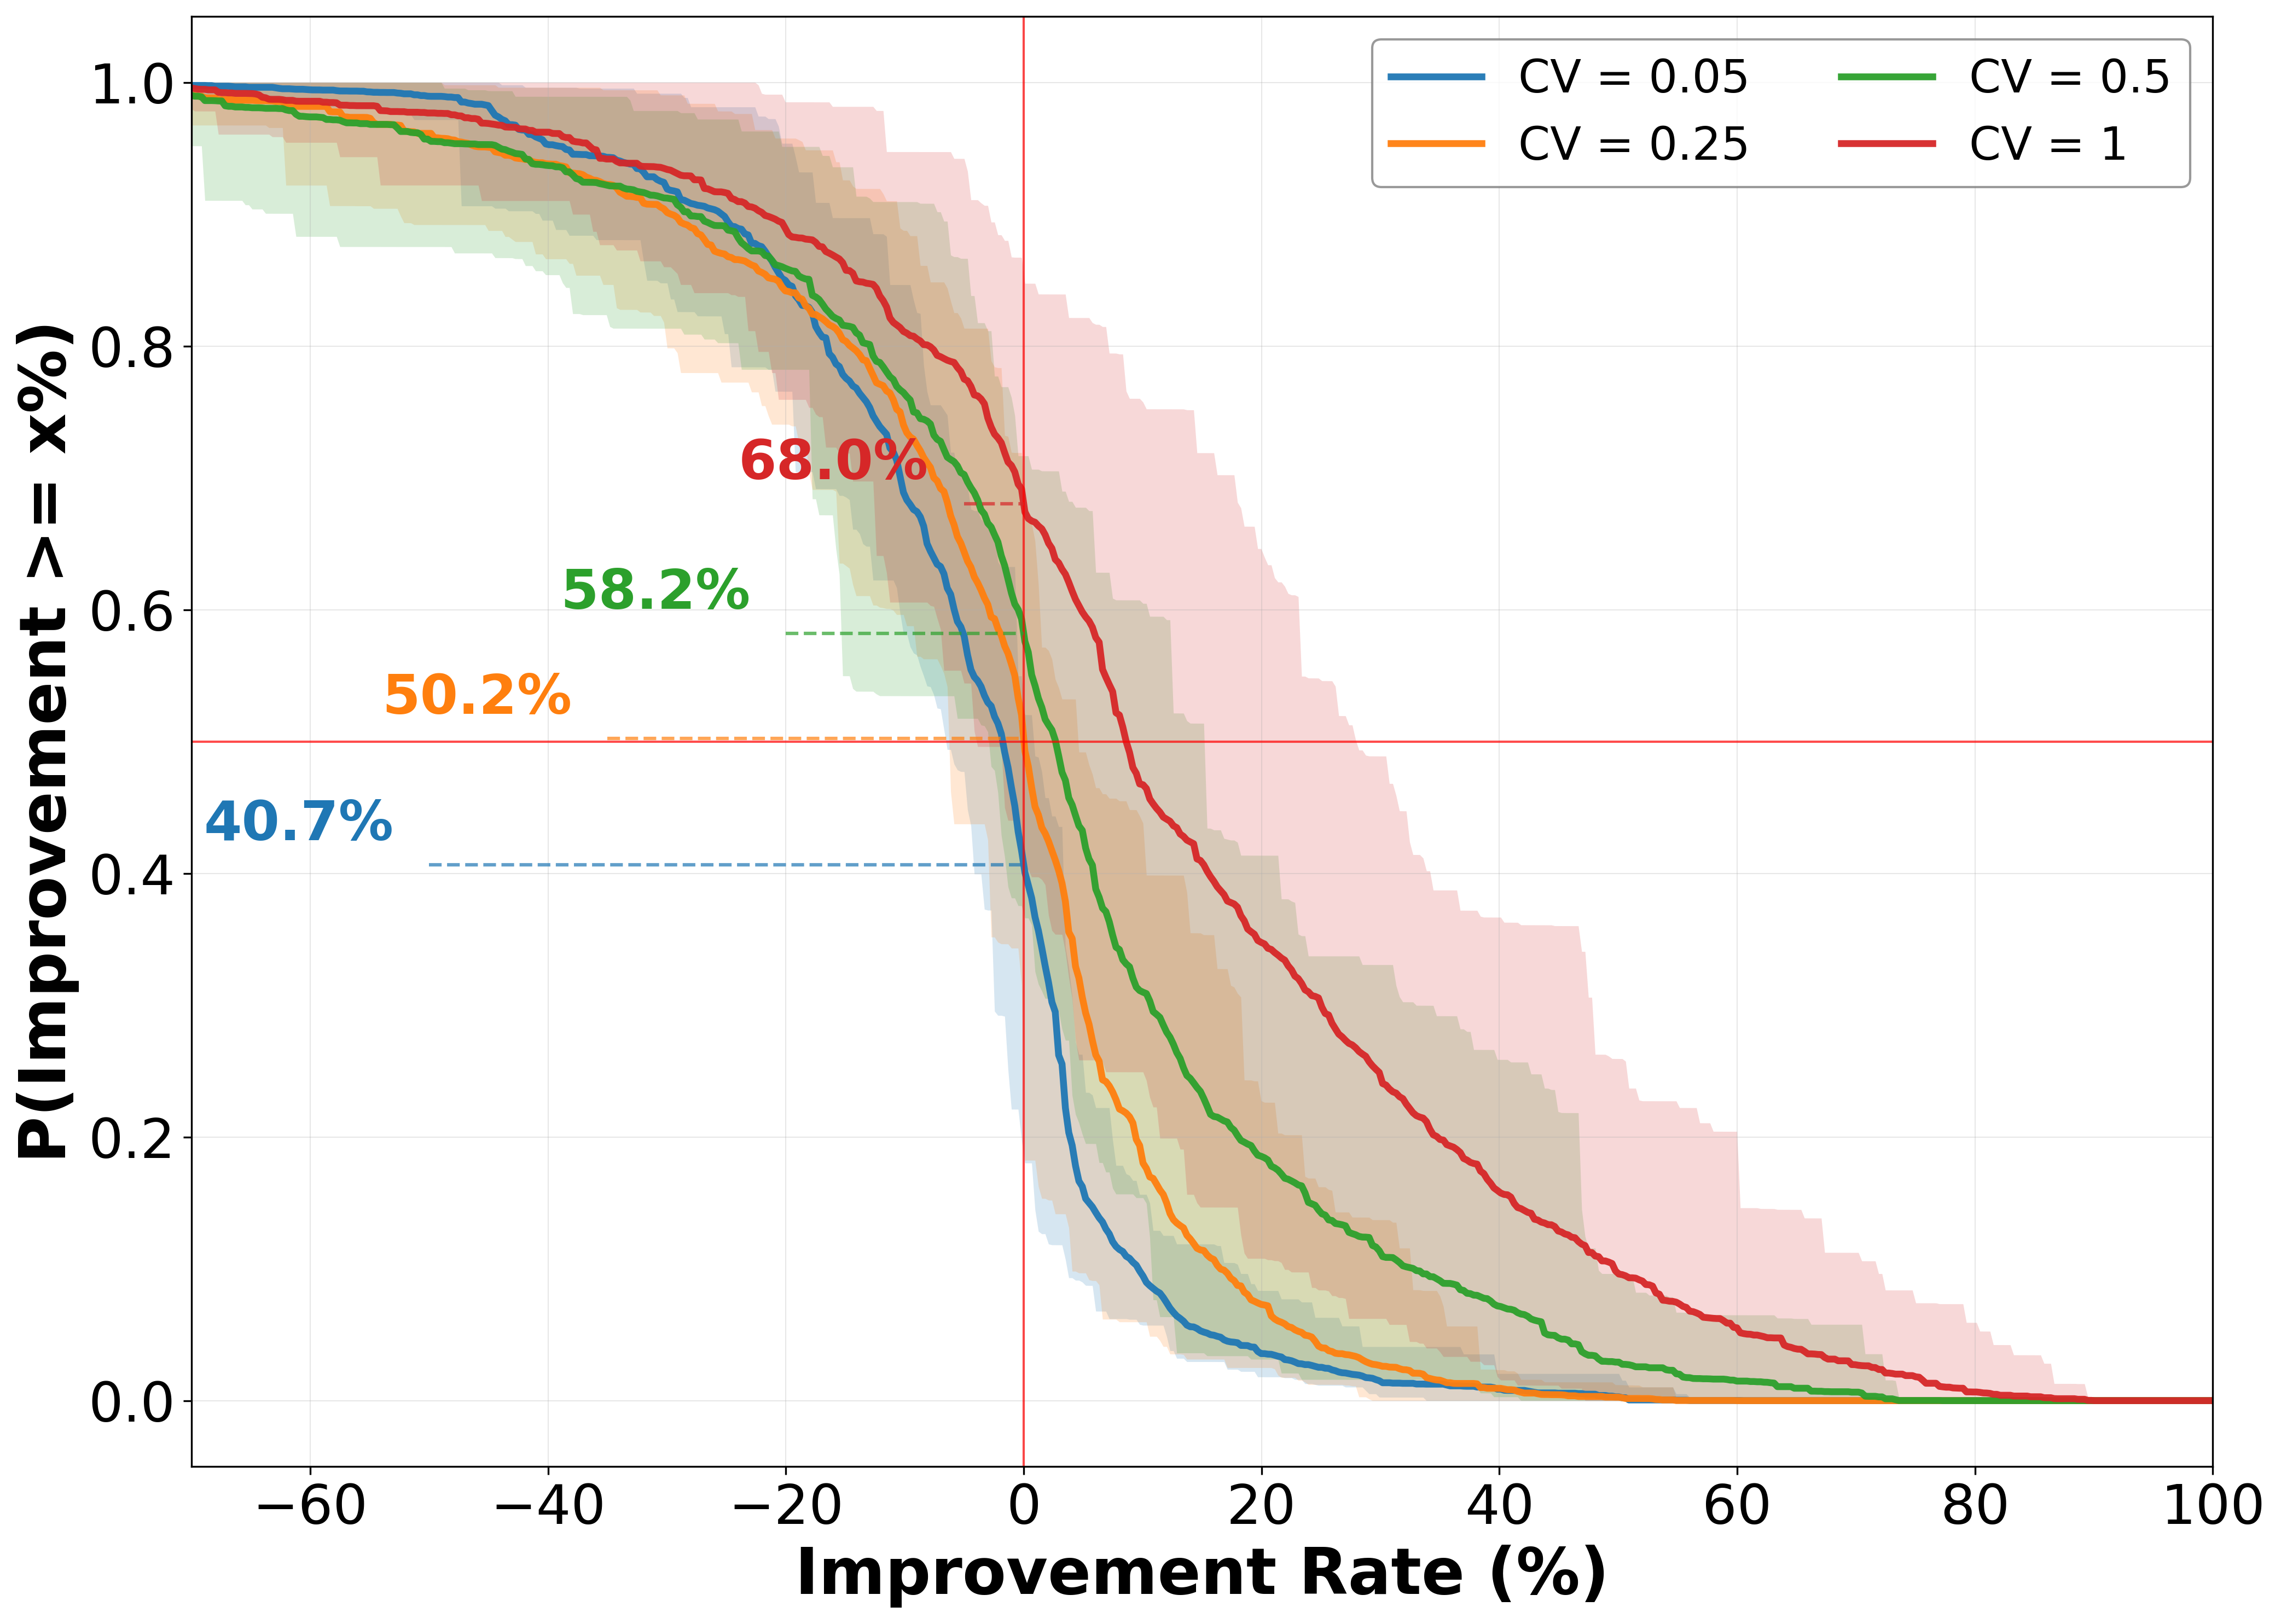
\includegraphics[width=\textwidth]{Fig/Analysis/D.1/improvement_icdf_6routes_all_cvs_trimmed_range.png}
        \caption{6 lines}
        \label{fig:appendix_improvement_exceedance_6routes}
    \end{subfigure}
    
    \medskip
    \begin{subfigure}[t]{0.47\textwidth}
        \centering
        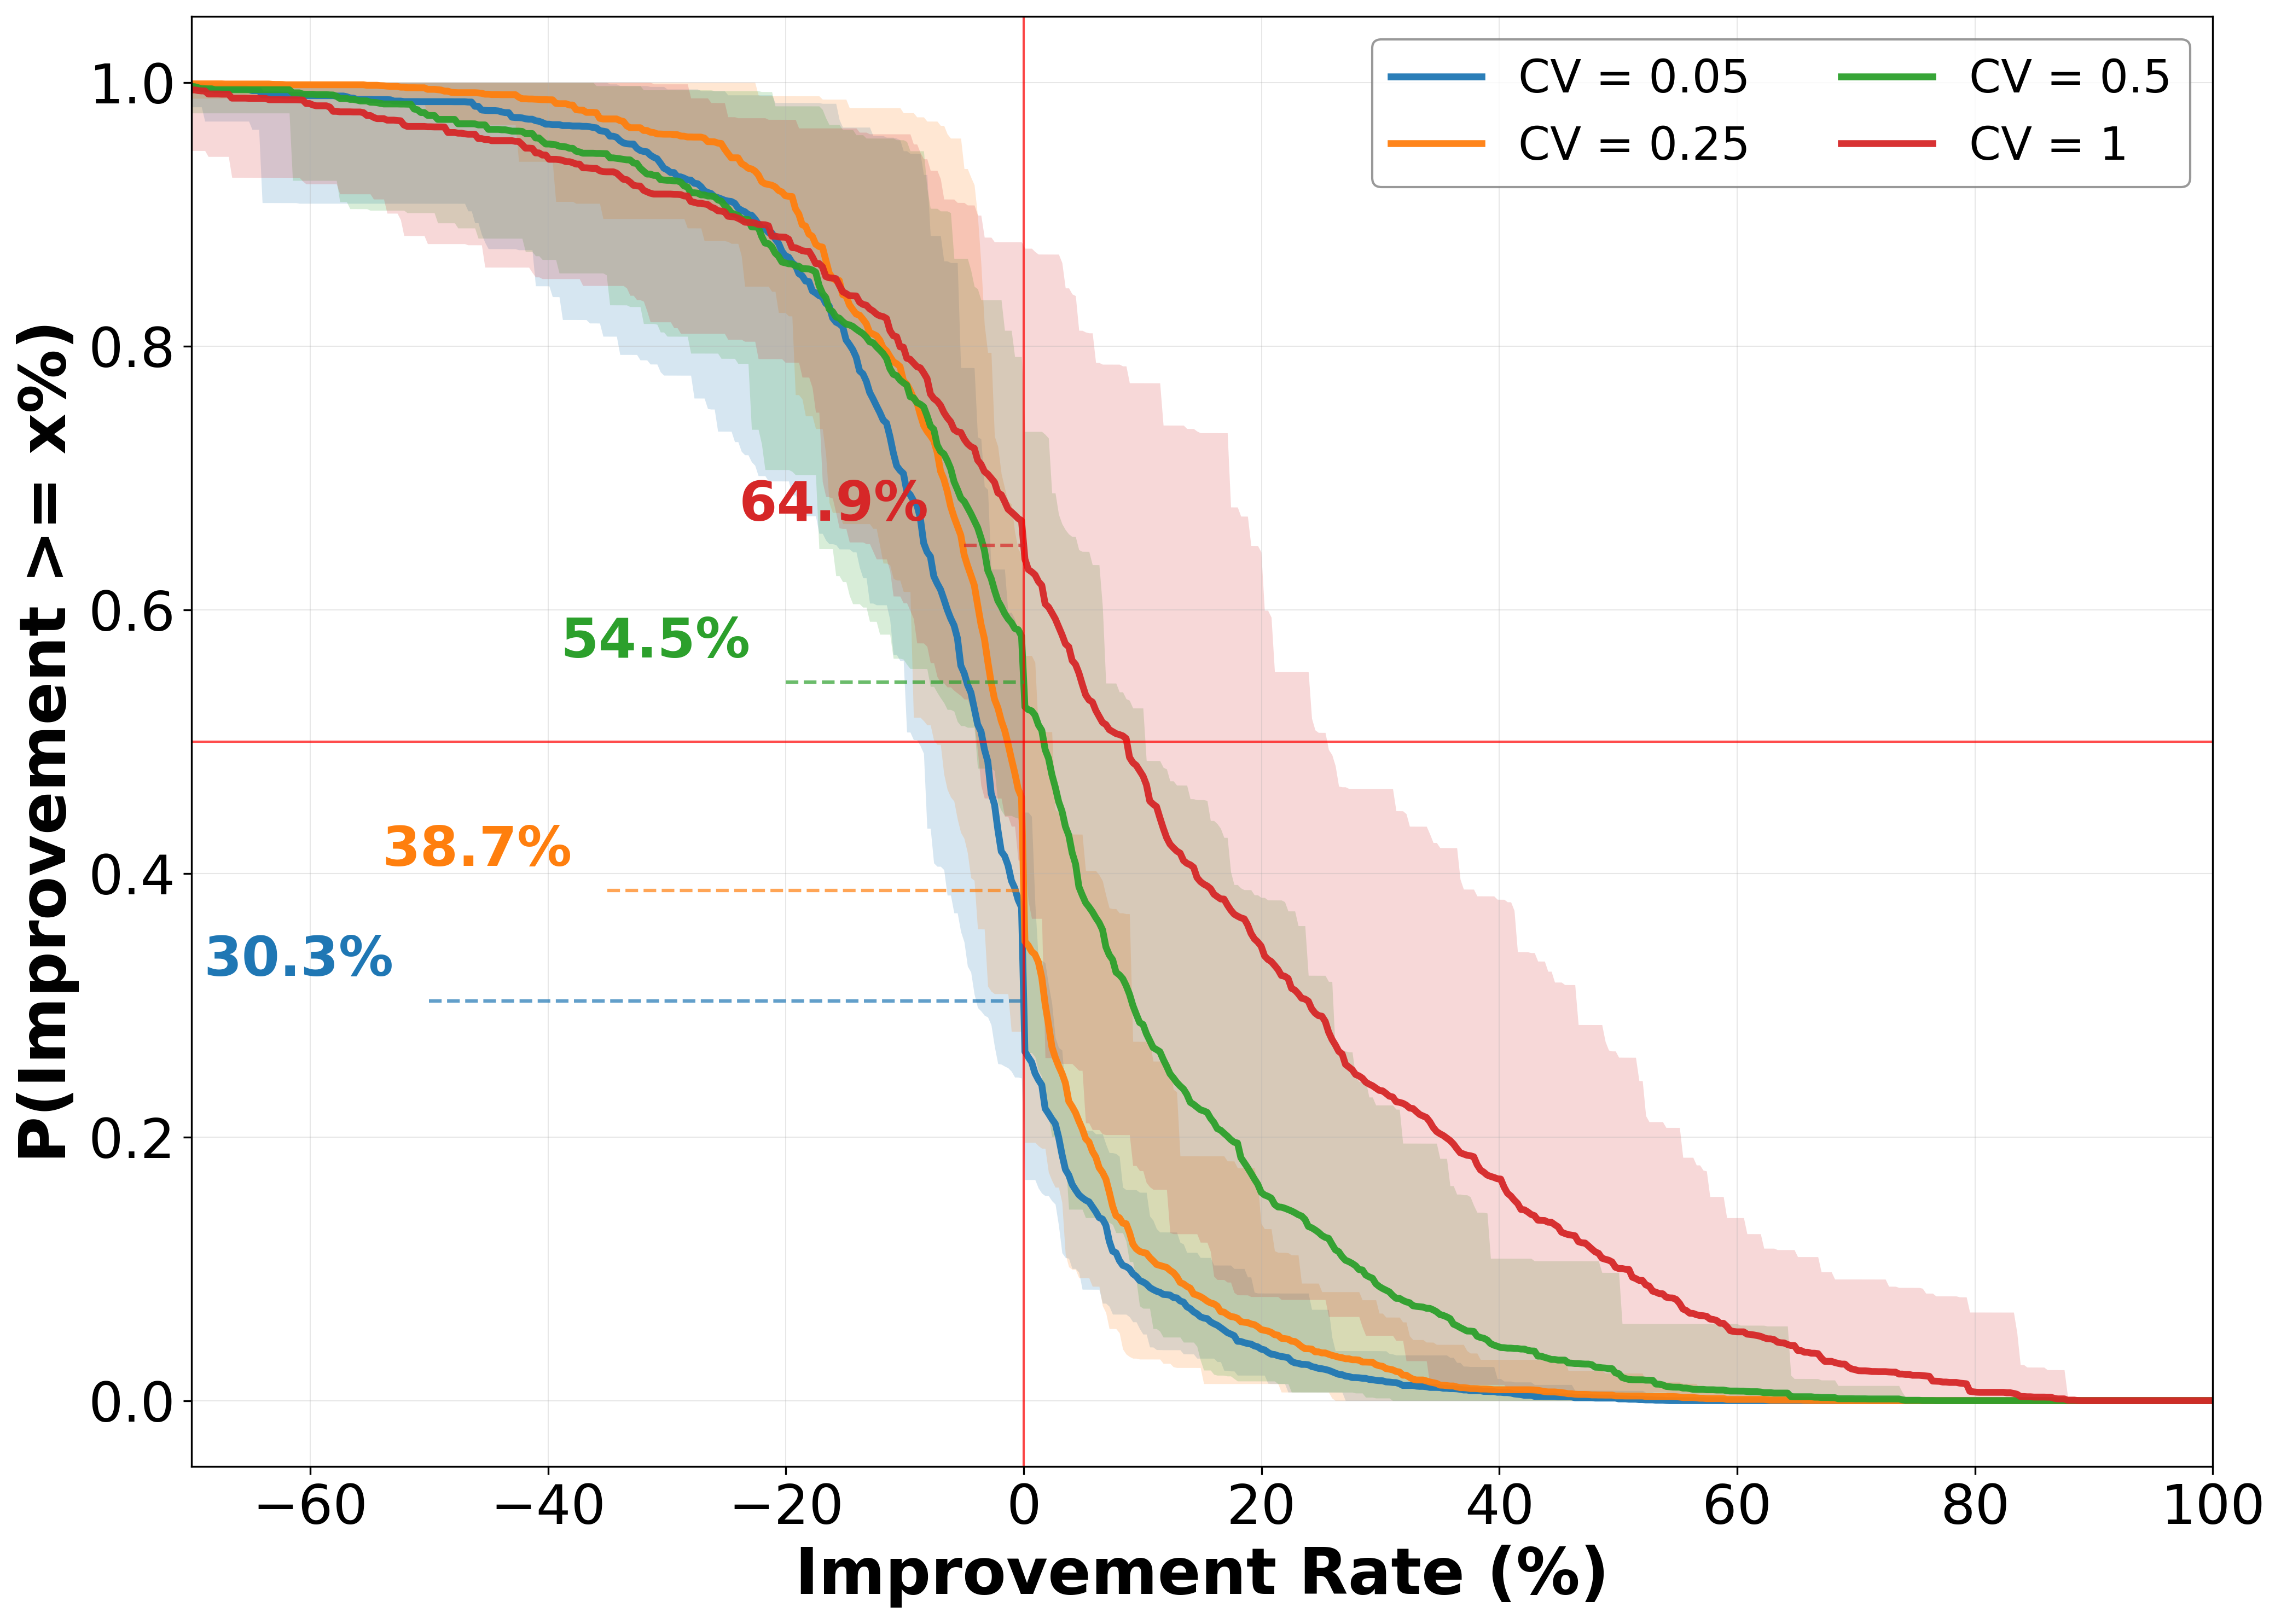
\includegraphics[width=\textwidth]{Fig/Analysis/D.1/improvement_icdf_8routes_all_cvs_trimmed_range.png}
        \caption{8 lines}
        \label{fig:appendix_improvement_exceedance_8routes}
    \end{subfigure}
    \hfill
    \begin{subfigure}[t]{0.47\textwidth}
        \centering
        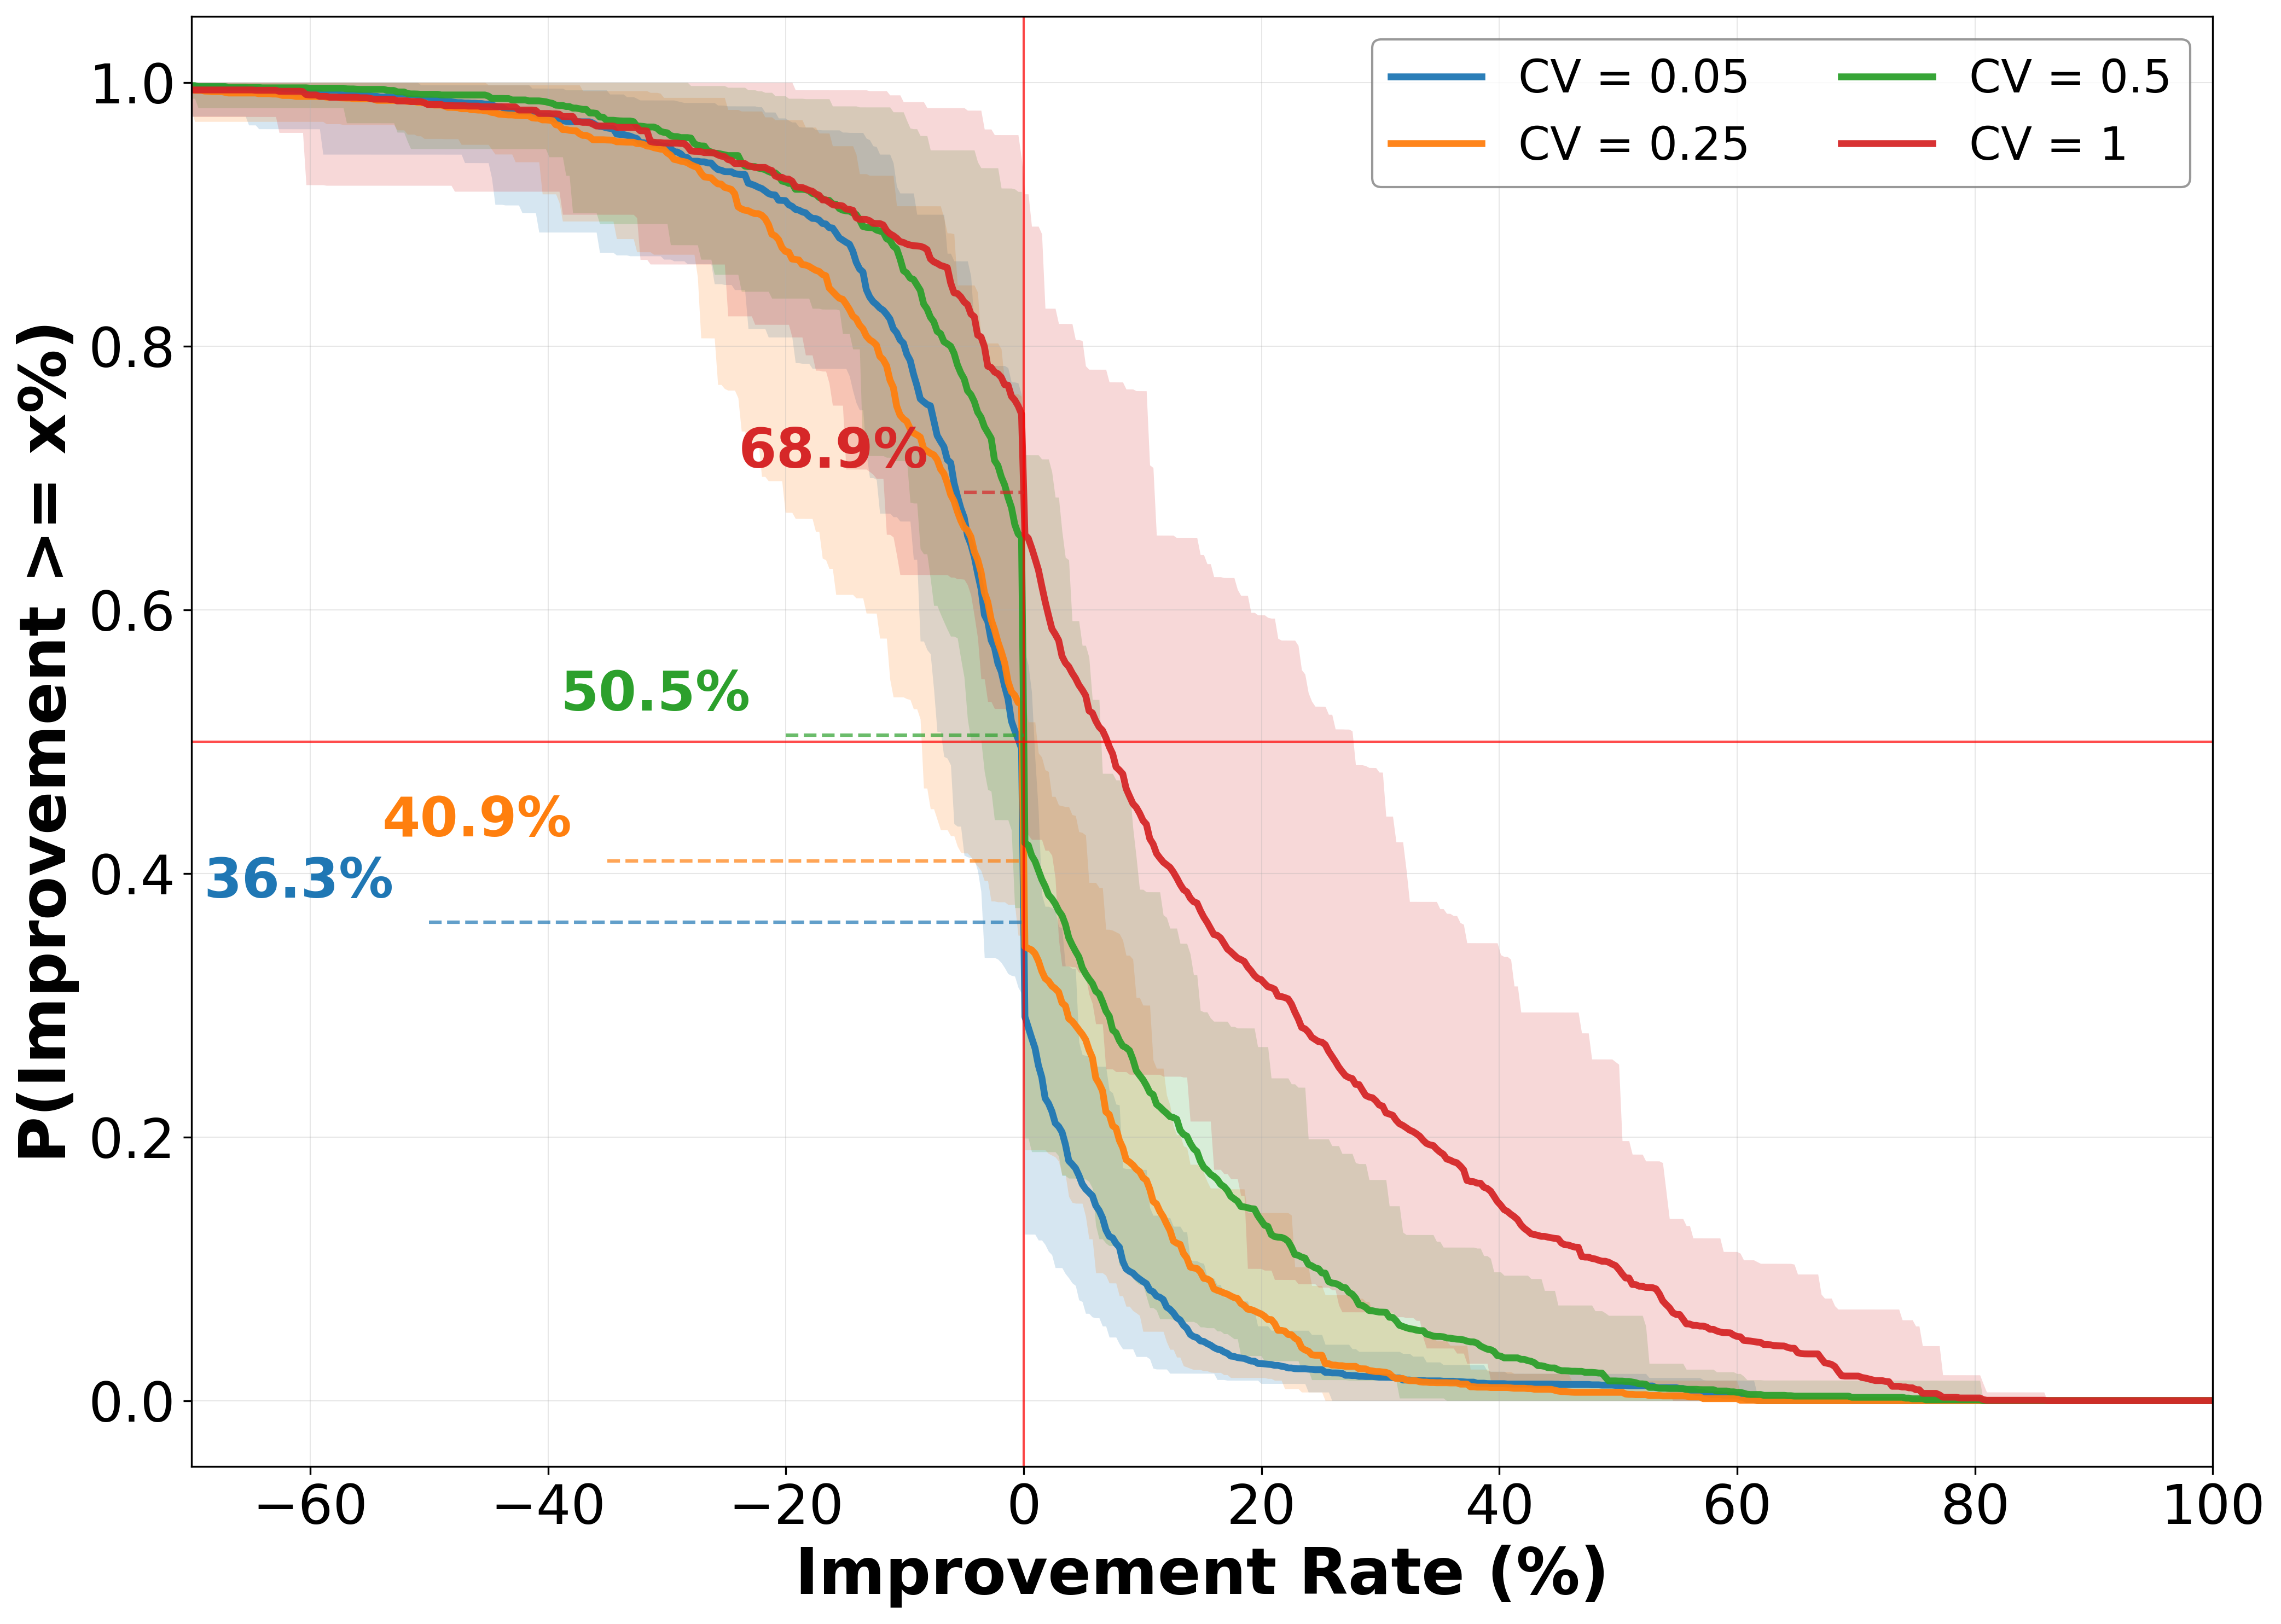
\includegraphics[width=\textwidth]{Fig/Analysis/D.1/improvement_icdf_10routes_all_cvs_trimmed_range.png}
        \caption{10 lines}
        \label{fig:appendix_improvement_exceedance_10routes}
    \end{subfigure}
    
    \medskip
    \begin{subfigure}[t]{0.47\textwidth}
        \centering
        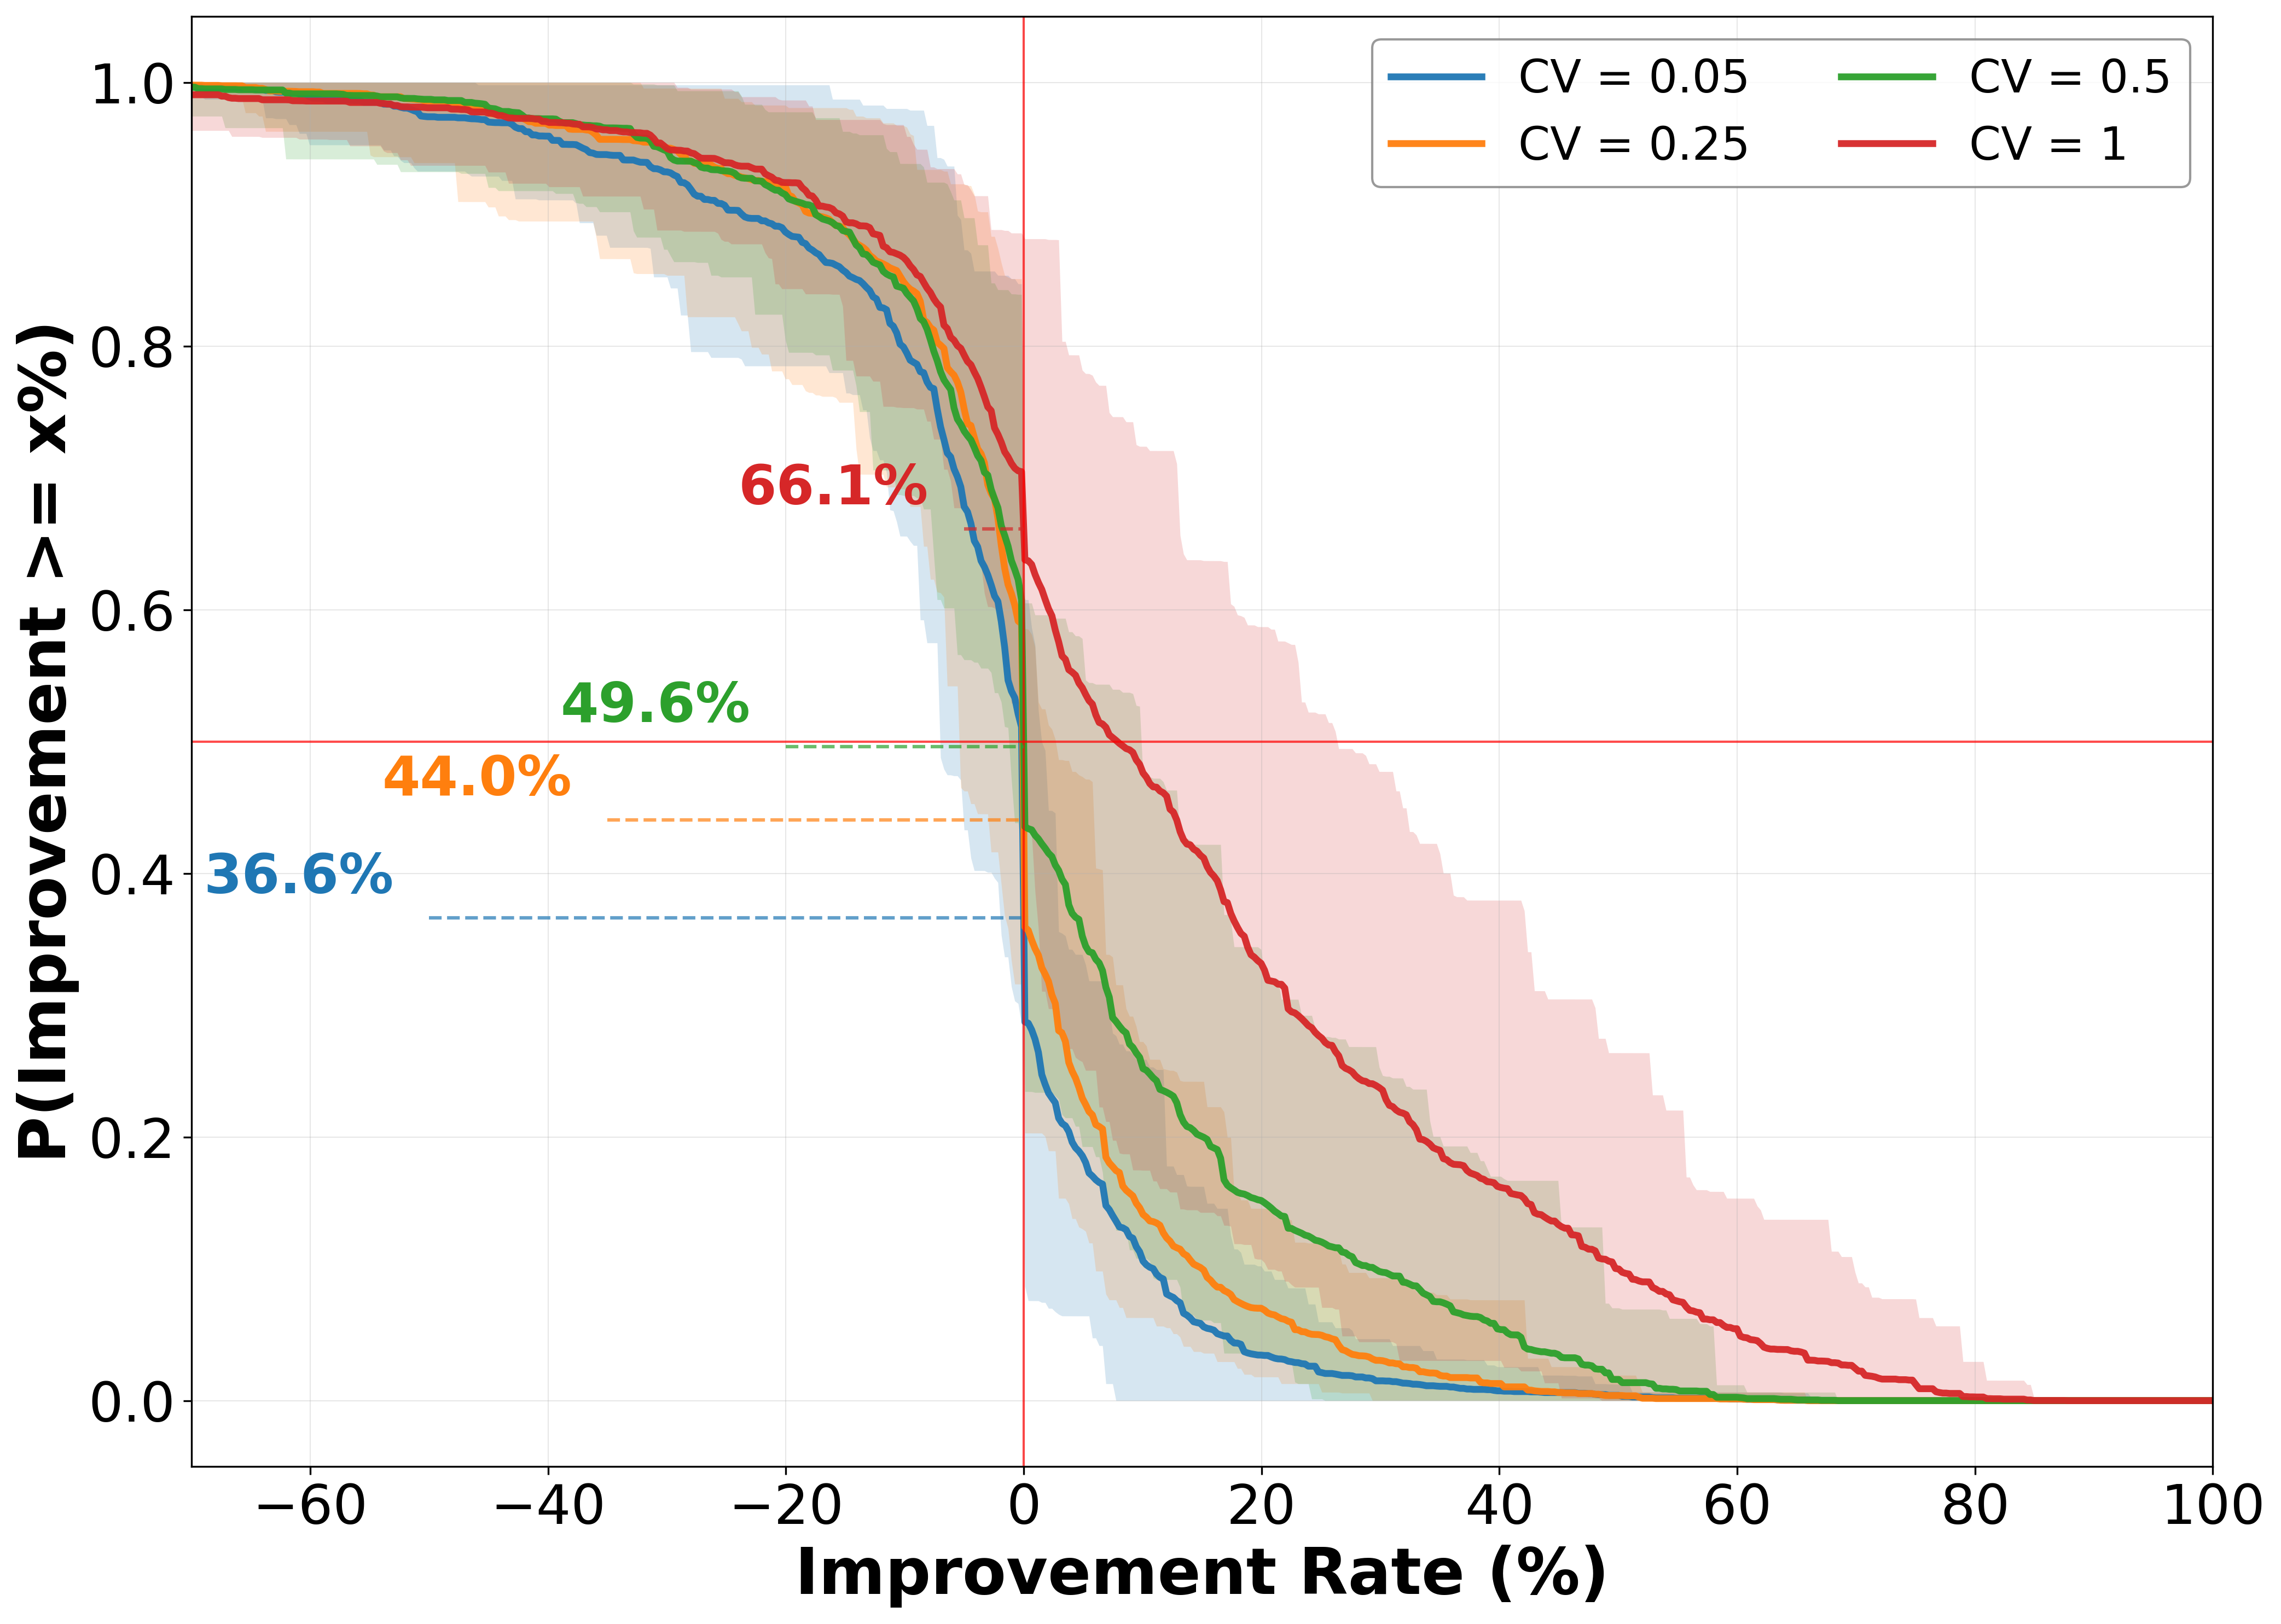
\includegraphics[width=\textwidth]{Fig/Analysis/D.1/improvement_icdf_12routes_all_cvs_trimmed_range.png}
        \caption{12 lines}
        \label{fig:appendix_improvement_exceedance_12routes}
    \end{subfigure}

    \caption{\rev{zg}{}{Trimmed-mean exceedance probability curves of OD-level improvement rates under different line quantities and variability levels. Each line is computed by first forming one per-seed quantile curve $Q_\omega(p)$ and then averaging the remaining curves after trimming extreme seed curves.}}
    \label{fig:appendix_improvement_exceedance_all_routes}
\end{center}

\section{Additional Beijing Network Visualisations}\label{app:beijing_networks}

\rev{zg}{}{Fig.~\ref{fig:app:beijingAllNetworks} complements the Beijing case-study visualisation by reporting the original network and the adapted line layouts at intermediate variability levels. These additional panels show that the redesign remains spatially targeted as $cv$ increases: lines are adjusted around affected corridors while preserving the broad structure of the original service network.}

\begin{center}
\captionsetup{type=figure}
\centering
\begin{subfigure}[t]{0.48\textwidth}
    \centering
    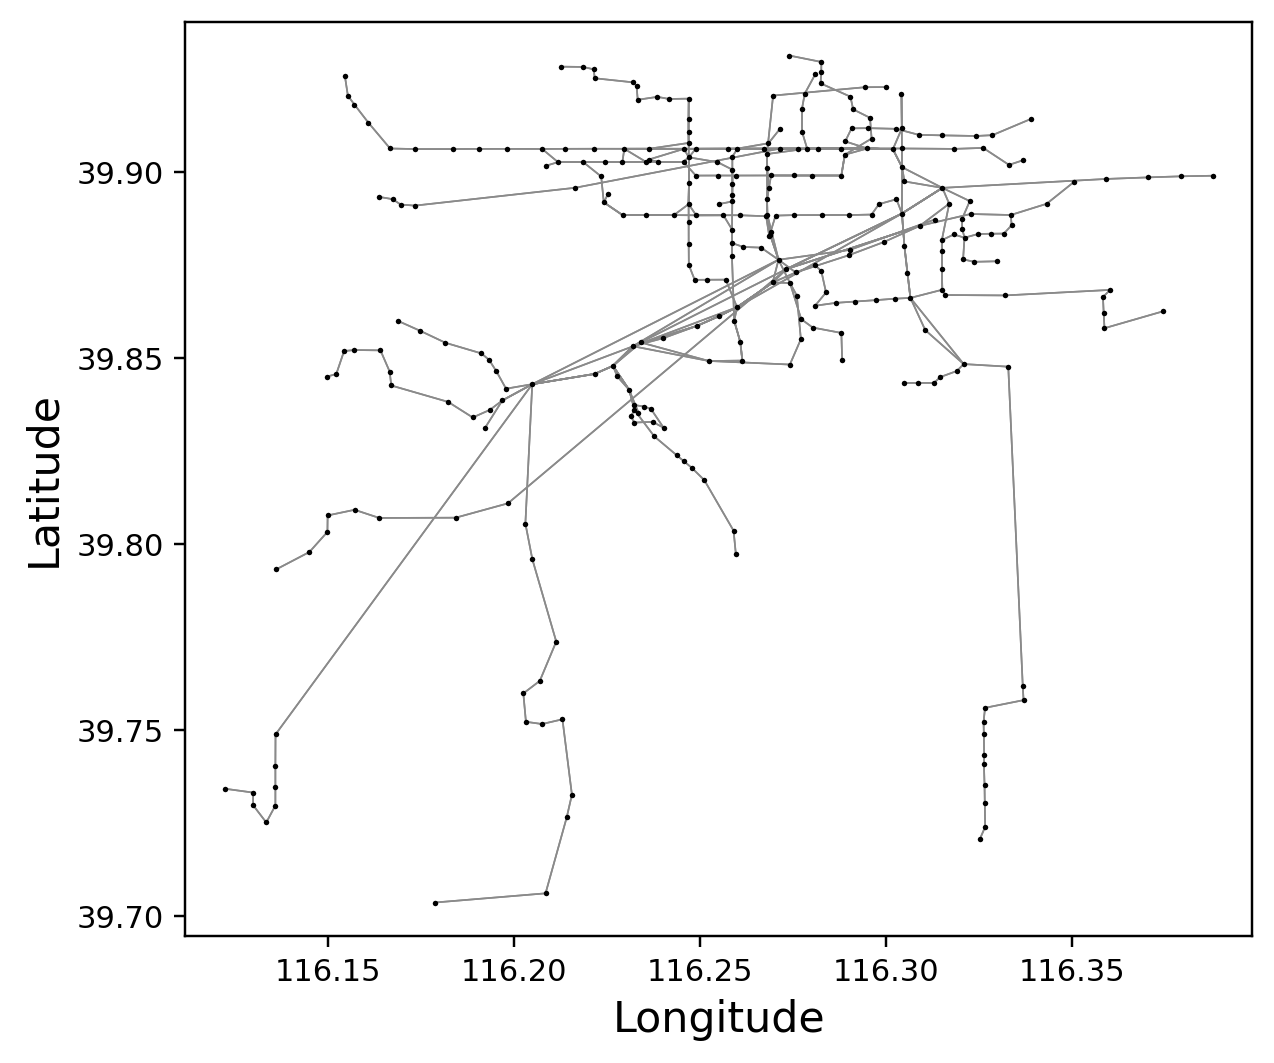
\includegraphics[width=\linewidth]{Fig/Case-Study/Beijing/Beijing1_original.png}
    \caption{Original network}
    \label{fig:app:beijingOriginal}
\end{subfigure}
\hfill
\begin{subfigure}[t]{0.48\textwidth}
    \centering
    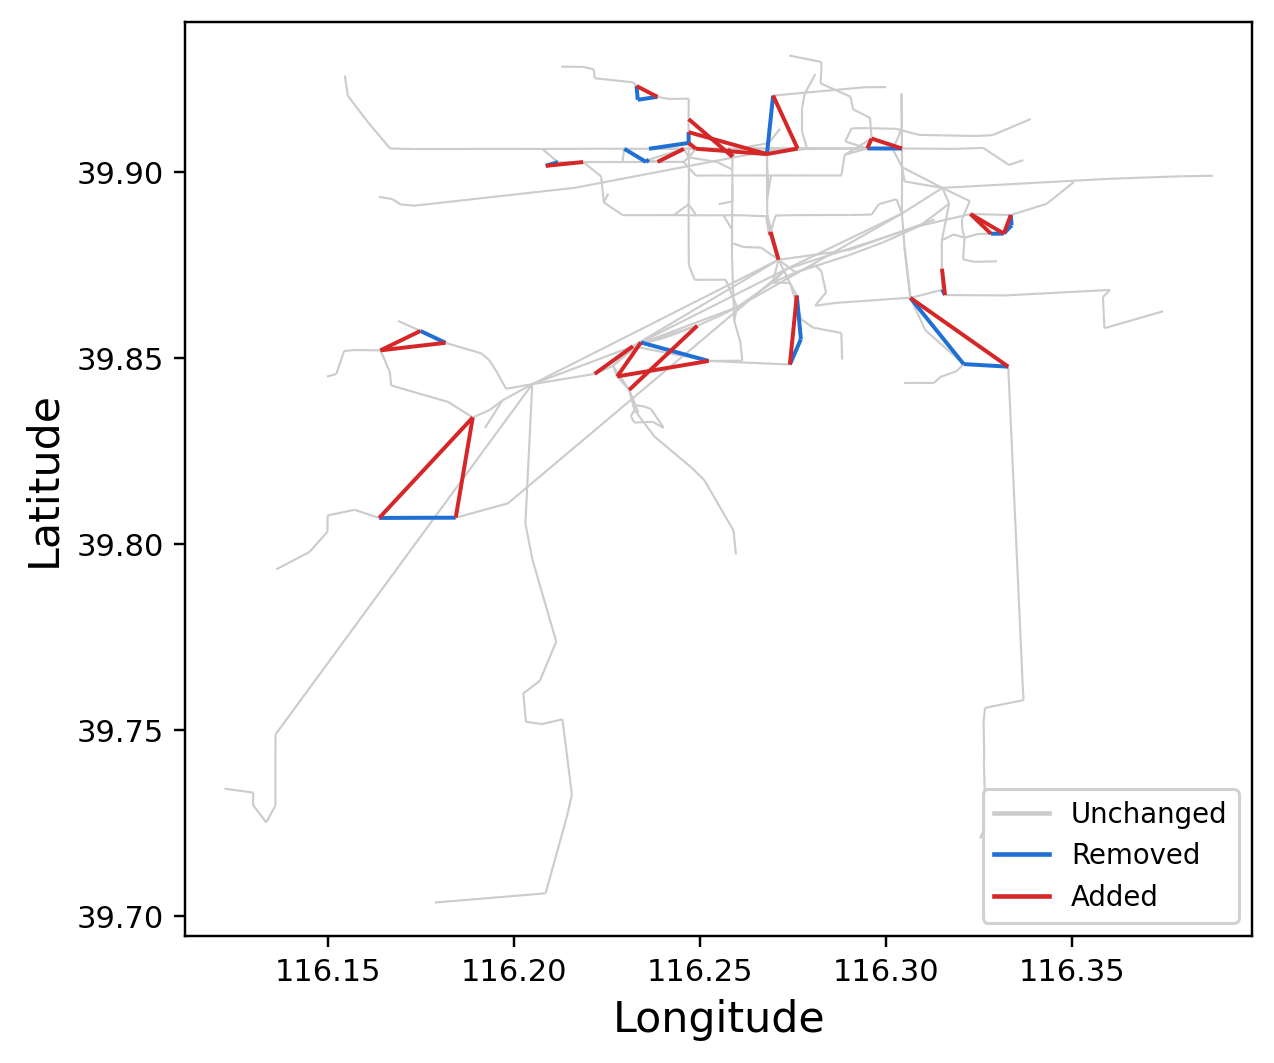
\includegraphics[width=\linewidth]{Fig/Case-Study/Beijing/Beijing_seed99_cv0p05.png}
    \caption{$cv = 0.05$}
    \label{fig:app:beijingCV0p05}
\end{subfigure}

\vspace{1em}

\begin{subfigure}[t]{0.48\textwidth}
    \centering
    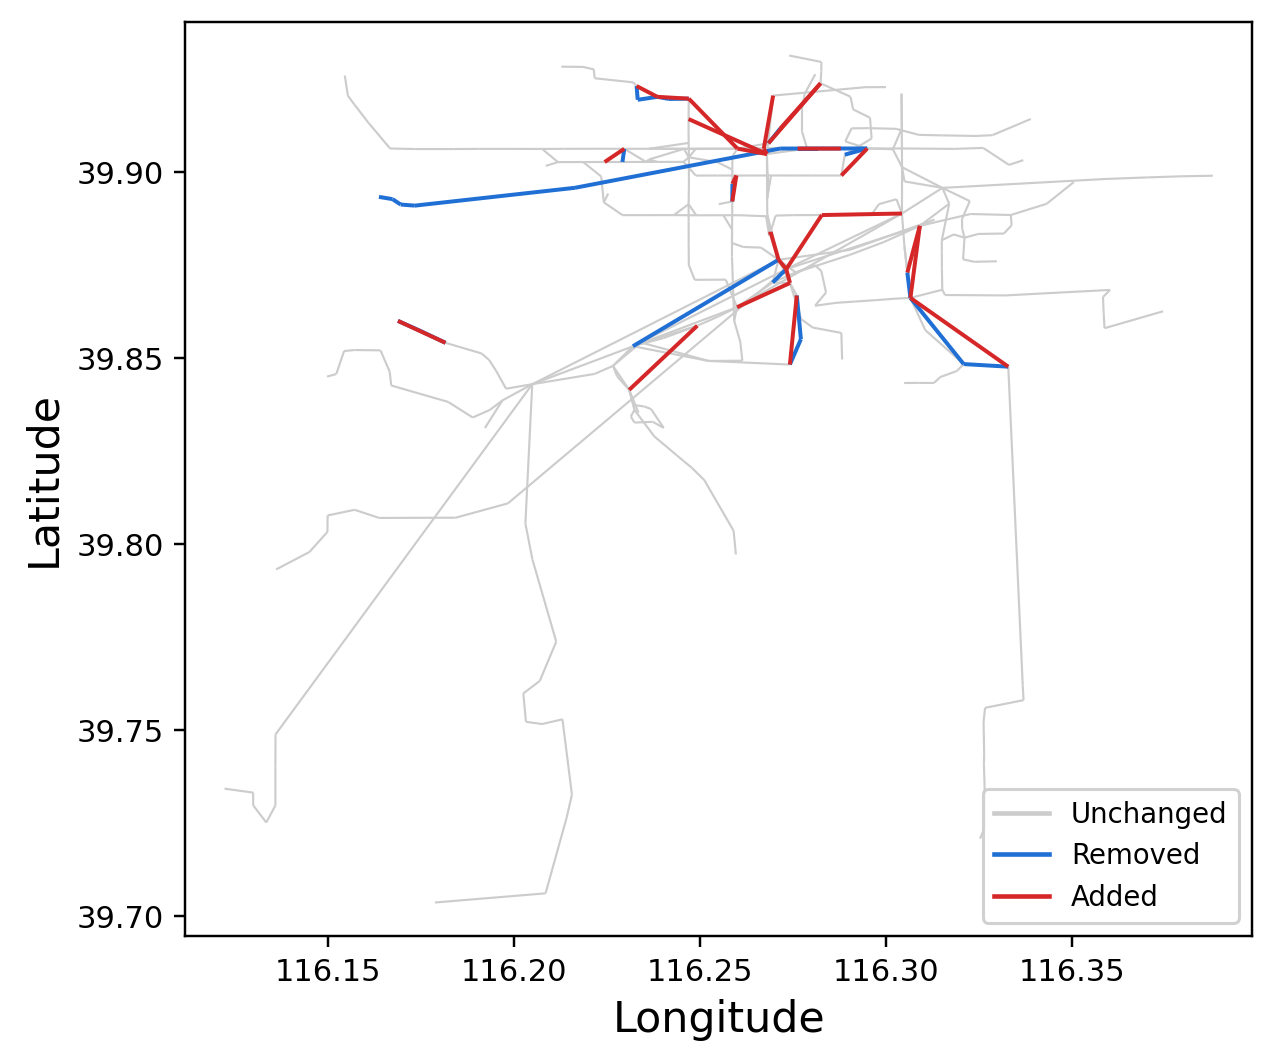
\includegraphics[width=\linewidth]{Fig/Case-Study/Beijing/Beijing_seed99_cv0p25.png}
    \caption{$cv = 0.25$}
    \label{fig:app:beijingCV0p25}
\end{subfigure}
\hfill
\begin{subfigure}[t]{0.48\textwidth}
    \centering
    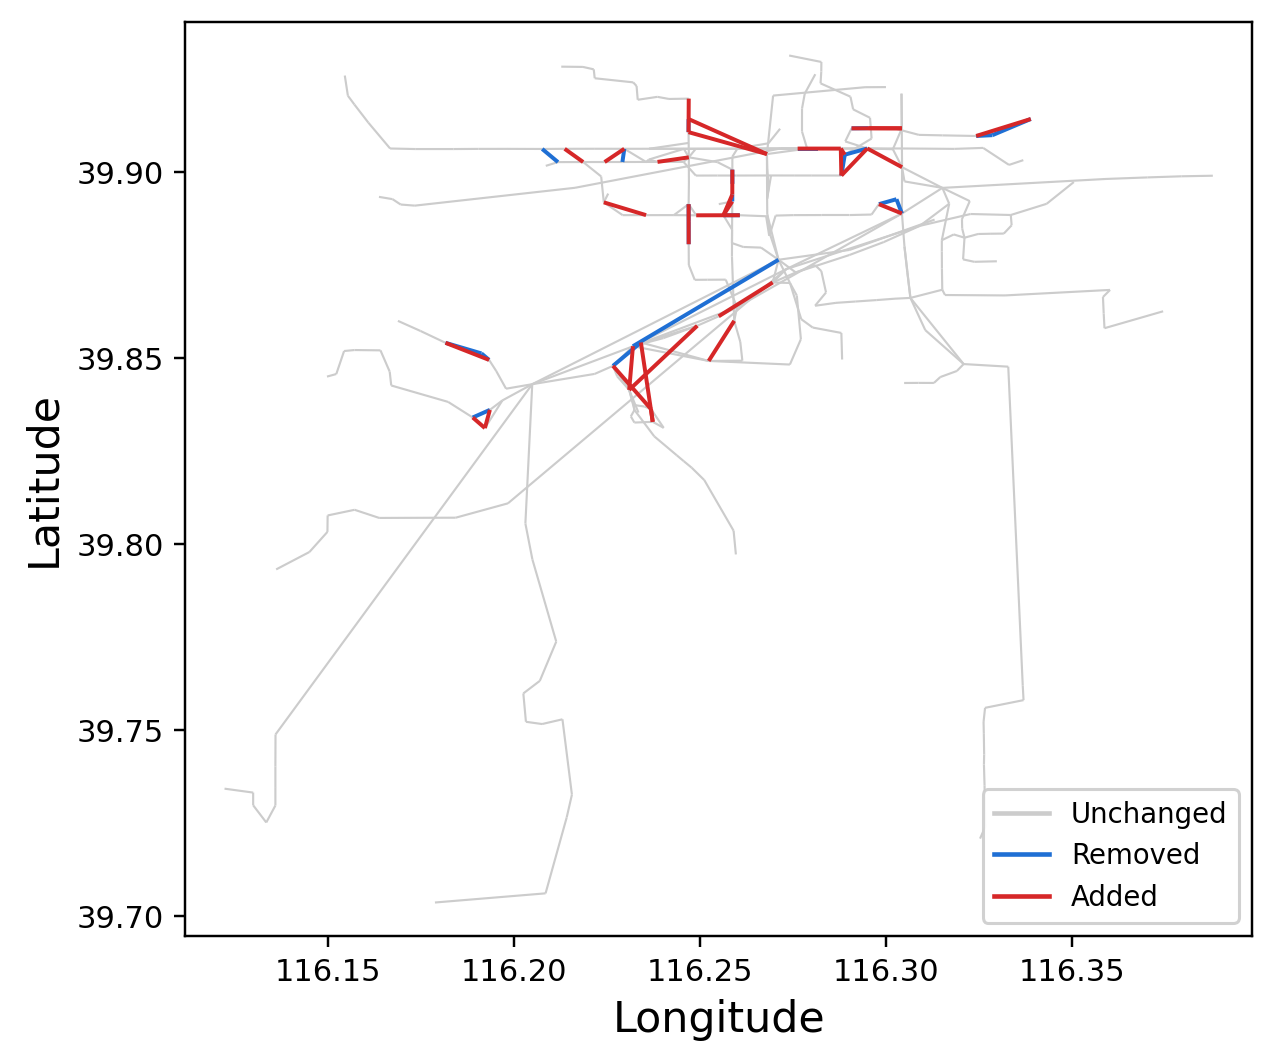
\includegraphics[width=\linewidth]{Fig/Case-Study/Beijing/Beijing_seed99_cv0p5.png}
    \caption{$cv = 0.5$}
    \label{fig:app:beijingCV0p5}
\end{subfigure}
\caption{\rev{zg}{}{Beijing PT networks: original design and adapted networks under $cv \in \{0.05, 0.25, 0.5\}$.}}
\label{fig:app:beijingAllNetworks}
\end{center}

%%%%%%%%%%%%%%%%%
\bibliographystyle{cas-model2-names}
\bibliography{cas-refs}
\end{document}
